\chapter{Parallel Monte Carlo Synthetic \\ Acceleration Methods\ }
\label{ch:parallel_methods}

In this chapter we briefly review particle transport methods for
domain decomposed Monte Carlo. Considering a domain decomposed
Neumann-Ulam method, we derive an analytic framework based on
algebraic quantities from which to estimate aspects of its performance
when applied to neutron transport systems. We then devise a parallel
algorithm for the Neumann-Ulam method based on the multiple-set
overlapping-domain decomposition algorithm and a parallel algorithm
for the MCSA iteration that leverages the parallel Monte Carlo
algorithm and general parallel matrix-vector operations. Using
parallel solutions for the neutron diffusion problem, we verify the
correctness of the parallel algorithm and implementation by comparing
the numerical results against production Krylov methods. With the
verified implementation of the algorithm, we perform parallel scaling
studies to test its performance on a leadership class machine and
compare this performance to the production Krylov methods.

%%---------------------------------------------------------------------------%%
\section{Domain Decomposed Monte Carlo\ }
\label{sec:msod}
Large-scale problems will for reasons typically related to memory
restrictions or performance have their data partitioned such that each
parallel process owns a subset of the equations in the linear
system. Given this convention, the Neumann-Ulam Monte Carlo algorithm
must perform random walks over a domain that is decomposed and must
remain decomposed to avoid the same performance and memory
restrictions that required the domain to be decomposed. To parallelize
this algorithm, we then seek parallel Monte Carlo algorithms that
handle domain decomposition.

To motivate this problem, consider the square domain presented in
Figure~\ref{fig:ddmc_example} and on this domain we imagine a Monte
Carlo particle transport problem. If the domain were decomposed into 9
subdomains as shown, each of those subdomains and their associated
data (i.e. cross sections) could be owned by a different parallel
process in the computation. In Figure~\ref{fig:ddmc_example}, the
tracks of 3 particles that are born in the center subdomain are
shown. In this example, particle A is first transported from the
center domain to the domain directly to the left. Before the
scattering event in the new domain may be processed, particle A must
be communicated between between the two parallel processes that own
those domains. For any given particle in the transport simulation,
this communication event may hardly occur during the lifetime of the
particle (particle B), or may occur many times (particle C) depending
on the problem parameters and the random path in phase space taken by
the particle. Scalable parallel algorithms for domain decomposed Monte
Carlo are those that handle this domain-to-domain communication of
particles effectively and balance it with the on-process computations
for particle interactions, tallies, response calculations, and other
simulation requirements.
\begin{figure}[t!]
  \begin{center}
    \scalebox{1.5}{
      \input{chapters/parallel_mc/ddmc_example.pdftex_t} }
  \end{center}
  \caption{\textbf{Domain decomposed Monte Carlo transport example
      illustrating how domain decomposition requires parallel
      communication of particles.} \textit{If a particle crosses a
      domain boundary it must be communicated to the next domain in
      its path.}}
  \label{fig:ddmc_example}
\end{figure}

For a domain decomposed Neumann-Ulam method, the situation is very
much the same where instead the transport process is now discrete and
the "physics" of the transport process is the Monte Carlo game with
probabilities and weights described by
Eq~(\ref{eq:neumann_ulam_decomposition}) for the given linear
problem. Figure~\ref{fig:ddnu_example} gives the domain decomposed
Neumann-Ulam analog of particle transport problem in
Figure~\ref{fig:ddmc_example}. Imagine in this problem that we are
solving for the monoenergetic scalar neutron flux as in the model
diffusion problem presented in Appendix~\ref{chap:diffusion_problem}.
In this problem, the solution has only a spatial dependence and
therefore each point in the mesh corresponds to an equation in the
resulting linear system. In Figure~\ref{fig:ddnu_example}, the domain
has now been discretized by this mesh and again decomposed into 9
subdomains, each owning a piece of the mesh and therefore the
corresponding equations in the linear system. As we play the Monte
Carlo game presented in Chapter~\ref{ch:stochastic_methods}, the
discretization and resulting Neumann-Ulam decomposition of the problem
describes how each state in the system is coupled to the other states
in the system through the set of equations that form the linear
system. This coupling is then responsible for the discrete random walk
that each history takes as shown in this example. As discrete states
(or rows in the linear system) that do not exist in the local domain
are reached during the random walk by stochastic histories, the
histories must be communicated to the subdomain that does own the
discrete state in an analogous fashion to the particles in the
previous example.
\begin{figure}[t!]
  \begin{center}
    \scalebox{1.5}{
      \input{chapters/parallel_mc/ddnu_example.pdftex_t} }
  \end{center}
  \caption{\textbf{Domain decomposed Neumann-Ulam example illustrating
      how domain decomposition requires parallel communication of
      histories.} \textit{Each mesh point corresponds to an equation
      in the linear system and the coupling among equations is
      described by the discretization of the problem.}}
  \label{fig:ddnu_example}
\end{figure}

To further motivate using a parallel algorithm similar to particle
transport methods, again consider history A in
Figure~\ref{fig:ddnu_example}. This history begins in the center
subdomain and through the course of transitioning through states in
the system arrives at a state that exists in the subdomain directly to
the left of the center subdomain. History A must then be communicated
from the center subdomain to the subdomain immediately to the left to
continue the random walk. As with the particle transport system, we
may find that histories in a domain decomposed Neumann-Ulam method are
only communicated a few times (history B) if at all, or they may be
communicated many times (history C) depending on the discretization
and the outcome of the Monte Carlo game. In identical fashion to the
particle transport problem, a domain decomposed Neumann-Ulam method
has the same communication requirements with all histories in both
examples requiring the same parallel operations. The amount of
communication of histories from domain to domain will be the primary
factor in the parallel scalability of the algorithm. In the next
section, the number of histories communicated in a given problem will
be quantified analytically for a simple model problem.

\clearpage

%%---------------------------------------------------------------------------%%
\section{Analytic Framework for Domain-Decomposed Monte Carlo\ }
\label{sec:analytic_framework}
To date, parallel Neumann-Ulam methods have been limited to full
domain replication with parallelism exploited through individual
histories \cite{alexandrov_efficient_1998} and in this chapter we
will exploit particle transport algorithms to alleviate this. To
accomplish this, we recognize from the literature that stochastic
histories must be transported from domain to domain as the simulation
progresses and they transition to states that are not in the local
domain. Because we have chosen a domain decomposition strategy in a
parallel environment, this means that communication of these histories
must occur between compute nodes owning neighboring pieces of the
global domain. We wish to characterize this communication not only
because communication is in general expensive, but also because these
nearest-neighbor communication sequences, specifically, have poor
algorithmic strong scaling \cite{gropp_high-performance_2001} in much
the same way as a parallel matrix-vector multiply
operation. Therefore, we desire a framework to provide a simple,
analytic theory based on the properties of the transport system that
will allow for estimates of the domain decomposed behavior of the
Neumann-Ulam method in terms of the amount of information that must be
communicated.

When solving problems where the linear operator is symmetric, a host
of analytic techniques exist based on the eigenvalue spectrum of the
operator that characterize their behavior in the context of
deterministic linear solvers. Using past work, these techniques are
adapted to the domain decomposed Neumann-Ulam method using the
one-speed, two-dimensional neutron diffusion equation and spatial
discretization presented in Appendix~\ref{chap:diffusion_problem} as a
model transport problem. Using the linear system generated by the
discretization of the model problem, we use a spectral analysis to
generate analytic relations for the eigenvalues of the operator based
on system parameters. Using the eigenvalue spectra, we then build
relationships to characterize the transport of stochastic histories in
a decomposed domain and the fraction of histories that leak from a
domain and will therefore have to be communicated. Finally, we compare
these analytic results to numerical experiments conducted with the
model transport problem.

\subsection{Spectral Analysis }
\label{subsec:spectral_analysis}
The convergence of the Neumann series in
Eq~(\ref{eq:adjoint_neumann_series}) approximated by the Monte Carlo
solver is dependent on the eigenvalues of the iteration matrix. We
will compute these eigenvalues by assuming eigenfunctions of the form
\cite{leveque_finite_2007}:
\begin{equation}
  \Phi_{p,q}(x,y) = e^{2 \pi \imath p x} e^{2 \pi \imath q y}\:,
  \label{eq:eigenfunction_form}
\end{equation}
where different combinations of $p$ and $q$ represent the different
eigenmodes of the solution. As these are valid forms of the solution,
then the action of the linear operator on these eigenfunctions will
yield the eigenvalues of the matrix as they exist on the unit circle
in the complex plane.

For the model problem, we first compute the eigenvalues for the
diffusion operator $\ve{D}$ by applying the operator to the
eigenfunctions and noting that $x=ih$ and $y=jh$:
\begin{multline}
  \ve{D}\Phi_{p,q}(x,y) = \lambda_{p,q}(\ve{D})
  =\\ -\frac{D}{6h^2}\Big[4 e^{-2 \pi \imath p h} + 4 e^{2 \pi \imath
      p h} + 4 e^{-2 \pi \imath q h} + 4 e^{2 \pi \imath q h} + e^{-2
      \pi \imath p h} e^{-2 \pi \imath q h} \\ + e^{-2 \pi \imath p h}
    e^{2 \pi \imath q h} + e^{2 \pi \imath p h} e^{-2 \pi \imath q h}
    + e^{2 \pi \imath p h} e^{2 \pi \imath q h} - 20\Big] + \Sigma_a
  \:.
  \label{eq:deriv_diff_1}
\end{multline}
Using Euler's formula, we can collapse the exponentials to
trigonometric functions:
\begin{equation}
  \lambda_{p,q}(\ve{D}) = -\frac{D}{6h^2}[ 8 \cos(\pi p h) + 8
    \cos(\pi q h) + 4 \cos(\pi p h) \cos(\pi q h) - 20] + \Sigma_a\:.
  \label{eq:deriv_diff_2}
\end{equation}

As Eq~(\ref{eq:diffusion_eq}) is diagonally dominant, point Jacobi
preconditioning as outlined in
\S~\ref{subsec:stochastic_preconditioning} is sufficient to reduce the
spectral radius of the iteration matrix below unity and therefore
ensure convergence of the Neumann series. Applying this
preconditioner, we are then solving the following diffusion system:
\begin{equation}
  \ve{M}^{-1} \ve{D} \boldsymbol{\phi} = \ve{M}^{-1} \ve{s}\:.
  \label{eq:precond_diffsion}
\end{equation}
The operator $\ve{M}^{-1} \ve{D}$ is merely the original diffusion
operator with each row scaled by the diagonal component. As we have
defined a homogeneous domain, the scaling factor, $\alpha$, is the
same for all rows in the operator and defined as the $\phi_{i,j}$
coefficient from Eq~(\ref{eq:fd_system}):
\begin{equation}
  \alpha = \Bigg[\frac{10 D}{3 h^2} + \Sigma_a\Bigg]^{-1}\:.
  \label{eq:jacobi_scaling}
\end{equation}
Using this coefficient, we then have the following spectrum of
preconditioned eigenvalues:
\begin{equation}
  \lambda_{p,q}(\ve{M}^{-1} \ve{D}) = \alpha \lambda_{p,q}(\ve{D})\:.
  \label{eq:preconditioned_eigenvalues}
\end{equation}

The spectral radius of the iteration matrix is obtained by seeking its
largest eigenvalue. As with the diffusion operator, we can use the
same analysis techniques to find the eigenvalues for the iteration
matrix. We use a few simplifications by noting that if the Jacobi
preconditioned iteration matrix is $\ve{H} = \ve{I} -
\ve{M}^{-1}\ve{D}$, the we except all terms on the diagonal of the
iteration matrix to be zero such that we have the following stencil:
\begin{multline}
  \ve{H}\boldsymbol{\phi} = \frac{\alpha D}{6h^2}\Big[4 \phi_{i-1,j} +
    4 \phi_{i+1,j} + 4 \phi_{i,j-1} + 4 \phi_{i,j+1}
    +\\ \phi_{i-1,j-1} + \phi_{i-1,j+1} + \phi_{i+1,j-1} +
    \phi_{i+1,j+1}\Big]\:.
  \label{eq:iteration_stencil}
\end{multline}
Inserting the eigenfunctions defined by
Eq~(\ref{eq:eigenfunction_form}) we get:
\begin{multline}
  \lambda_{p,q}(\ve{H}) = \frac{\alpha D}{6h^2}\Big[4 e^{-2 \pi \imath p
      h} + 4 e^{2 \pi \imath p h} + 4 e^{-2 \pi \imath q h} + 4 e^{2
      \pi \imath q h} + e^{-2 \pi \imath p h} e^{-2 \pi \imath q h}
    \\ + e^{-2 \pi \imath p h} e^{2 \pi \imath q q} + e^{2 \pi \imath
      p h} e^{-2 \pi \imath q h} + e^{2 \pi \imath p h} e^{2 \pi
      \imath q h}\Big]\:,
  \label{eq:iteration_deriv}
\end{multline}
which simplifies to:
\begin{equation}
  \lambda_{p,q}(\ve{H}) = \frac{\alpha D}{6h^2}[ 8 \cos(\pi p h) + 8
    \cos(\pi q h) + 4 \cos(\pi p h) \cos(\pi q h)]\:,
  \label{eq:iteration_spectrum}
\end{equation}
giving the eigenvalue spectrum for the Jacobi preconditioned iteration
matrix. We find that the maximum eigenvalue exists when $p=q=0$,
giving the following for the spectral radius of the Jacobi
preconditioned iteration matrix:
\begin{equation}
  \rho(\ve{H}) = \frac{10 \alpha D}{3 h^2}\:.
  \label{eq:iteration_radius}
\end{equation}

\subsection{Neumann Series Convergence }
\label{subsec:neumann_convergence}
As outlined in \S\ref{sec:mc_preliminaries}, the adjoint Monte Carlo
method is effectively an approximation to a stationary method. In the
adjoint Neumann-Ulam method, $k$ iterations, equivalent to $k$
applications of the iteration matrix, are approximated by a random
walk of average length $k$ to yield the summation in
Eq~(\ref{eq:adjoint_neumann_solution})
\cite{dimov_new_1998,danilov_asymptotic_2000}. This random walk
length, or the number of transitions before the termination of a
history (either by the weight cutoff, absorption, or exiting the
global domain) is therefore approximately the number of stationary
iterations required to converge to the specified tolerance. In the
case of the adjoint Neumann-Ulam method, no such tolerance exists,
however, we have specified a weight cutoff, $W_c$, that determines
when low-weight histories will be prematurely terminated as their
contributions are deemed minute. After $k$ iterations, a stationary
method is terminated as the error has reached some fraction,
$\epsilon$, of the initial error:
\begin{equation}
  ||\ve{e}^{k}||_2 = \epsilon ||\ve{e}^0||_2\:.
  \label{eq:linear_k_iter_norm4}
\end{equation}
Per Eq~(\ref{eq:linear_k_iter_norm3}), we see that this fraction is
equivalent to $\epsilon = \rho(\ve{H})^k$. For the adjoint
Neumann-Ulam method, if we take this fraction to be the weight cutoff,
a measure of how accurately the contributions of a particular history
to the solution are tallied, we then have the following relationship
for $k$:
\begin{equation}
  k = \frac{ \log(W_c) }{ \log( \rho(\ve{H}) ) }\:.
  \label{eq:analytic_k}
\end{equation}
This then gives us a means to estimate the length of the random walks
that will be generated from a particular linear operator based on the
eigenvalues of its iteration matrix (independent of the linear
operator splitting chosen) and based on the weight cutoff parameter
used in the Neumann-Ulam method.

\subsection{Domain Leakage Approximations }
\label{subsec:domain_leak_approx}
In a domain decomposed situation, not all histories will remain within
the domain they started in and must instead be communicated. This
communication, expected to be expensive, was analyzed by Siegel and
colleagues for idealized, load balanced situations for full nuclear
reactor core Monte Carlo neutral particle simulations
\cite{siegel_analysis_2012}.  To quantify the number of particles
that leak out of the local domain they define a leakage fraction,
$\Lambda$, as:
\begin{equation}
  \Lambda = \frac{average\ \#\ of\ particles\ leaving\ local\ domain}
          {total\ of\ \#\ of\ particles\ starting\ in\ local\ domain}\:.
          \label{eq:leakage_fraction}
\end{equation}
For their studies, Siegel and colleagues assumed that the value of
$\Lambda$ was dependent on the total cross section of the system via
the Wigner rational approximation. Outlined more thoroughly by Hwang's
chapter in \cite{azmy_nuclear_2010}, we will use both the Wigner
rational approximation and the mean chord approximation as a means to
estimate the leakage fraction.

In the case of domain decomposed linear systems, we can use diffusion
theory to estimate the optical thickness of a domain in the
decomposition and the corresponding leakage fraction in terms of
properties of the linear operator and the discretization. To begin we
must first calculate the mean distance a Monte Carlo history will move
in the grid by computing the mean squared distance of its movement
along the chord of length $l$ defined across the domain. After a
single transition a history will have moved a mean squared distance
of:
\begin{equation}
  \langle \bar{r_1^2} \rangle = (n_s h)^2\:,
  \label{eq:step_1_length}
\end{equation}
where $h$ is the size of the discrete grid elements along the chord
and $n_s$ is the number of grid elements a history will move on
average every transition. For our diffusion model problem, $n_s$ would
equate to the expected number of states in the $i$ (or $j$ as the problem is
symmetric) direction that a history will move in a single
transition and is dependent on the stencil used for the
discretization. After $k$ transitions in the random walk, the history
will have moved a mean squared distance of:
\begin{equation}
  \langle \bar{r_k^2} \rangle = k (n_s h)^2\:.
  \label{eq:step_k_length}
\end{equation}
If our chord is of length $l$ and there are $n_i$ grid elements (or
states to which a history may transition) along that chord, then $h =
l / n_i$ giving:
\begin{equation}
  \langle \bar{r_k^2} \rangle = k \Bigg(\frac{n_s l}{n_i}\Bigg)^2\:.
  \label{eq:step_k_length_sub}
\end{equation}
From diffusion theory, we expect the average number of interactions
along the chord to be:
\begin{equation}
  \tau = \frac{l}{2 d \sqrt{\langle \bar{r_k^2} \rangle}}\:,
  \label{eq:optical_thickness_1}
\end{equation}
where $d$ is the dimensionality of the problem and $\sqrt{\langle
  \bar{r_k^2} \rangle}$ is effectively the mean free path of the Monte
Carlo history in the domain. We can readily interpret $\tau$ to be the
\textit{effective optical thickness} of a domain of length
$l$. Inserting Eq~(\ref{eq:step_k_length_sub}) we arrive at:
\begin{equation}
  \tau = \frac{n_i}{2 d n_s \sqrt{k}}\:,
  \label{eq:optical_thickness_2}
\end{equation}
which if expanded with Eq~(\ref{eq:analytic_k}) gives us the final
relation for the effective optical thickness:
\begin{equation}
  \tau = \frac{n_i}{2 d n_s}
  \sqrt{\frac{\log(\rho(\ve{H}))}{\log(W_c)}}\:.
  \label{eq:optical_thickness_3}
\end{equation}

For optically thin domains, we expect that most histories will be
communicated, while optically thick domains will leak the fraction of
histories that did not interact within. Using the optical thickness
defined in Eq~(\ref{eq:optical_thickness_3}), we can then complete the
leakage approximations by defining the bounds of $\tau \rightarrow 0,
\Lambda \rightarrow 1$ and $\tau \rightarrow \infty, \Lambda
\rightarrow \tau^{-1}$.  With these bounds we can then define the
leakage fraction out of a domain for the adjoint Neumann-Ulam method
using the Wigner rational approximation:
\begin{equation}
  \Lambda = \frac{1}{1+\tau}\:,
  \label{eq:wigner_domain_leakage}
\end{equation}
and using the mean-chord approximation:
\begin{equation}
  \Lambda = \frac{1-e^{-\tau}}{\tau}\:.
  \label{eq:mean_chord_domain_leakage}
\end{equation}
Here, the leakage fraction is explicitly bound to the eigenvalues of
the iteration matrix, the size of the domain, the content of the
discretization stencil, and the weight cutoff selected to terminate
low weight histories.

\subsection{Numerical Experiments }
\label{subsec:numerical_experiments}
To test the relationships developed by the spectral analysis, we form
two simple numerical experiments using the diffusion model problem:
one to measure the length of the random walks as a function of the
iteration matrix eigenvalues, and one to measure the domain leakage
fraction as a function of the iteration matrix eigenvalues and the
discretization properties. Before doing this, we verify our
computation of the spectral radius of the iteration matrix by
numerically computing the largest eigenvalue of the diffusion operator
using an iterative eigenvalue solver. For this verification, a $100
\times 100$ square grid with $h=0.01$, $h=0.1$, and $h=1.0$ and the
absorption cross varied from 0 to 100 while the scattering cross
section was fixed at unity. Figure~\ref{fig:measured_spec_rad} gives
the measured spectral radius of the iteration matrix and the computed
spectral radius for the preconditioned diffusion operator using
Eq~(\ref{eq:iteration_radius}) as function of the absorption to
scattering ratio $(\Sigma_a / \Sigma_s)$. Excellent agreement was
observed between the analytic and numerical results with all data
points computed within the tolerance of the iterative eigenvalue
solver.
\begin{figure}[t!]
  \begin{spacing}{1.0}
    \begin{center}
      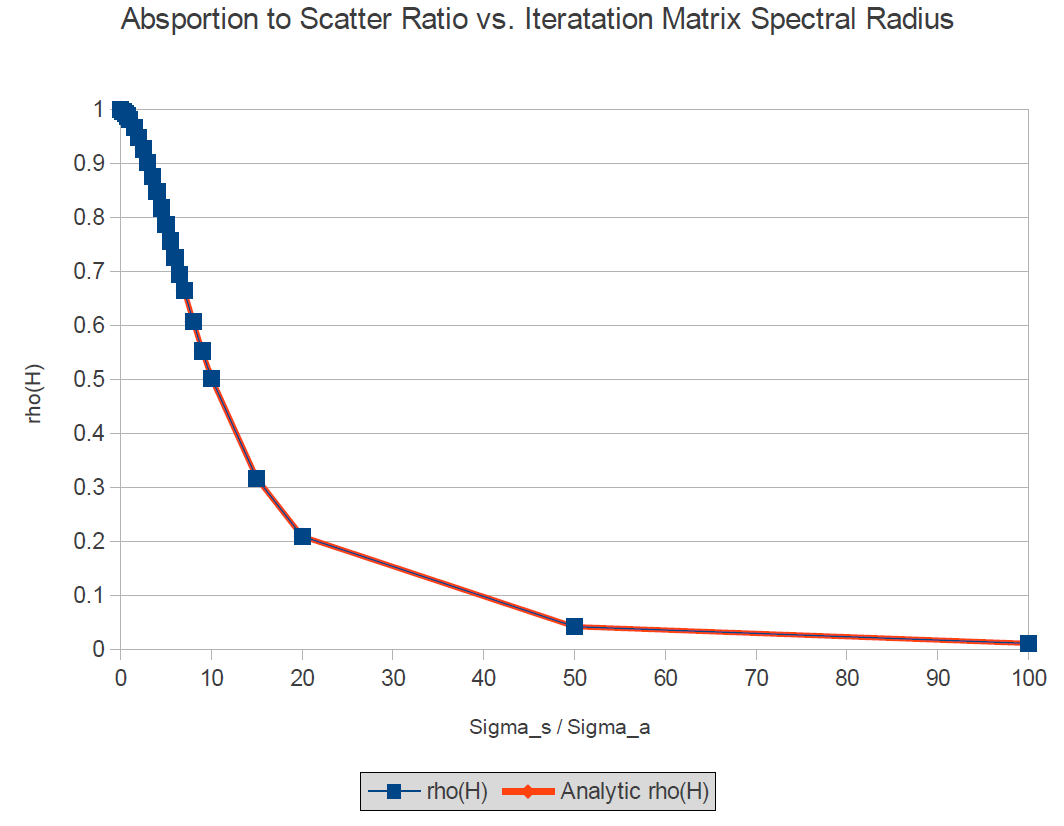
\includegraphics[width=4in,clip]{chapters/parallel_mc/measured_spec_rad.png}
    \end{center}
    \caption{\textbf{Measured and analytic preconditioned diffusion
        operator spectral radius as a function of the absorption cross
        section to scattering cross section ratio.} \textit{Values of
        $h=0.01$, $h=0.1$, and $h=1.0$ were used. The red data was
        computed numerically by an eigensolver while the black dashed
        data was generated by Eq~(\ref{eq:iteration_radius}).}}
    \label{fig:measured_spec_rad}
  \end{spacing}
\end{figure}

\subsubsection{Random Walk Length }
\label{subsubsec:walk_length}
With the eigenvalue derivations verified, we can go about setting up
an experiment to measure the length of the random walks generated by
the adjoint Neumann-Ulam solver. To do this, we again use a $100
\times 100$ square grid with $h=0.1$ and the absorption cross varied
from 0 to 100 while the scattering cross section was fixed at
unity. Three weight cutoff values of \sn{1}{-2}, \sn{1}{-4}, and
\sn{1}{-8} were used with 10,000 histories generated by a point source
of strength 1 in the center of the domain. For each of the histories,
the number of transitions made was tallied to provide an effective
value of $k$ for each history. This value was then averaged over all
histories to get a measured value of $k$ for the particular
operator. On the left, Figure~\ref{fig:measured_length} presents these
measurements as well as the analytic result computed by
Eq~(\ref{eq:analytic_k}) as a function of the iteration matrix
spectral radius, $\rho(\ve{H})$. On the right,
Figure~\ref{fig:measured_length} gives the relative difference between the
predicted and observed results. We note good qualitative agreement
between the measured and analytic results. However, we observe a
larger relative difference for both long and short random walks.
\begin{figure}[t!]
  \begin{spacing}{1.0}
    \begin{center}
      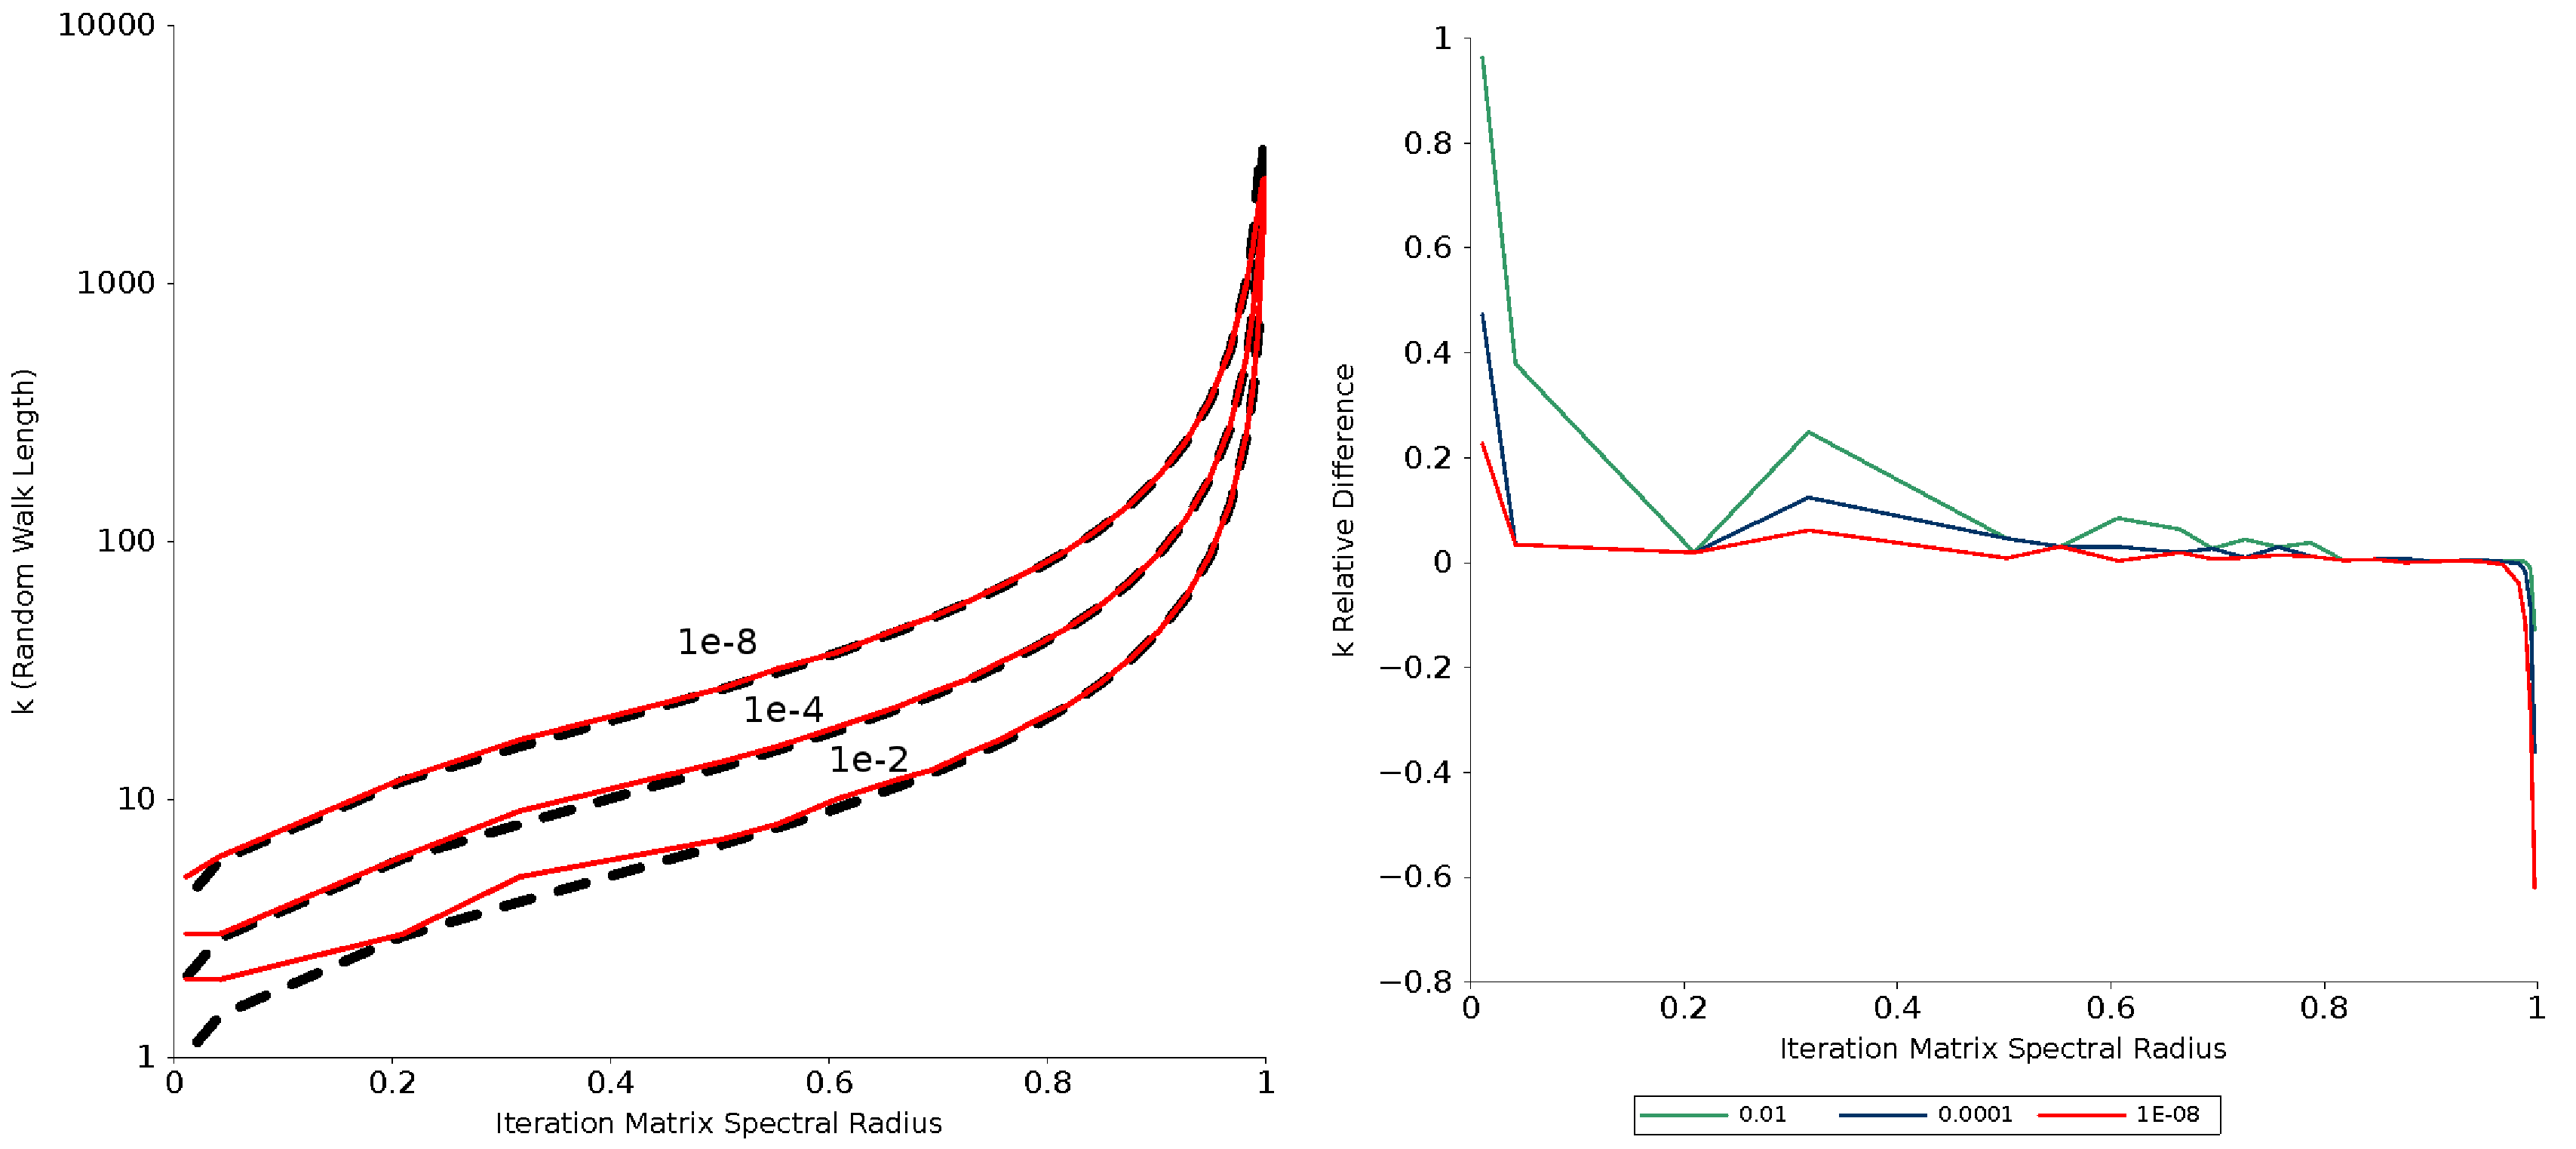
\includegraphics[width=6.0in,clip]{chapters/parallel_mc/measured_length_2.pdf}
    \end{center}
    \caption{\textbf{Measured and analytic random walk length as a
        function of the iteration matrix spectral radius.} \textit{The
        weight cutoff was varied with \sn{1}{-2}, \sn{1}{-4}, and
        \sn{1}{-8}. In the left plot, the red data was computed
        numerically by an adjoint Neumann-Ulam implementation while
        the black dashed data was generated by
        Eq~(\ref{eq:analytic_k}). In the right plot, the relative
        difference between the predicted and measured results is
        presented for each weight cutoff.}}
    \label{fig:measured_length}
  \end{spacing}
\end{figure}

\subsubsection{Domain Leakage }
\label{subsubsec:domain_leakage}
Finally, we seek to measure the leakage from a domain in a domain
decomposed Monte Carlo calculation and assess the quality of our
analytic relation for the optical thickness of a domain and the
associated leakage approximations. For this experiment, a square grid
with $h=0.1$ was decomposed into 9 square domains, 3 in each cardinal
direction with measurements occurring in the central domain without
boundary grid points. For the cross sections, the absorption cross
section was varied from 1 to 100 while the scattering cross
section was set to zero to create a purely absorbing environment
with weight cutoff of \sn{1}{-4}. The optical thickness of these
domains will vary as a function of the absorption cross section if
the other parameters are fixed. 

To compute the optical thickness, along with the spectral radius as
given by Eq~(\ref{eq:iteration_radius}), we also need the parameters
$n_i$ and $n_s$ which respectively describe the typical domain length
and the average number of states moved along that typical length per
history transition. For our grid above, the domains are varied in size
with $50 \times 50$, $100 \times 100$, and $200 \times 200$ cells
giving $n_i=50$, $n_i=100$, and $n_i=200$ grid points or states along
the typical length of the domain respectively. Looking at the
Laplacian stencil in Eq~(\ref{eq:nine_point_stencil}), we see that all
history transitions will only move a single state in either the $i$ or
$j$ directions due to the symmetry of the problem. Furthermore, if we
choose the $i$ direction, not all states we will transition to will
move the history in that direction. Therefore, we look to the
definition of the iteration matrix in Eq~(\ref{eq:iteration_stencil})
and the definition of the adjoint probability matrix in
Eq~(\ref{eq:adjoint_probability}) to estimate the $n_s$ parameter. For
a particular transition starting at state $(i,j)$, 6 of the 8 possible
new states in the stencil move the history in $i$ direction with
relative coefficients of 4 for moving in the $(\pm i,0)$ direction and
of 1 for moving in the $(\pm i,\pm j)$. These coefficients dictate the
frequency those states are visited relative to the others. For those 6
states we can visit along the typical length, their sum is 12 out of
the total 20 for the coefficients for all possible states with their
ratio giving $n_s = \frac{3}{5}$.

To compute the leakage fraction numerically, \sn{3}{5} histories were
sampled from a uniform source of strength unity over the global
domain. At the start of a stage of histories, the number of histories
starting in the center domain was computed and as the stage
progressed, the number of histories that exited that domain was
tallied with the ratio of the two numbers providing a numerical
measure for the leakage fraction. Figure~\ref{fig:measured_leakage}
gives the domain leakage measurements for the domain in the center of
the global grid as well as the analytic result computed by
Eqs~(\ref{eq:wigner_domain_leakage}) and
(\ref{eq:mean_chord_domain_leakage}) as a function of the iteration
matrix spectral radius.
\begin{figure}[t!]
  \begin{spacing}{1.0}
    \begin{center}
      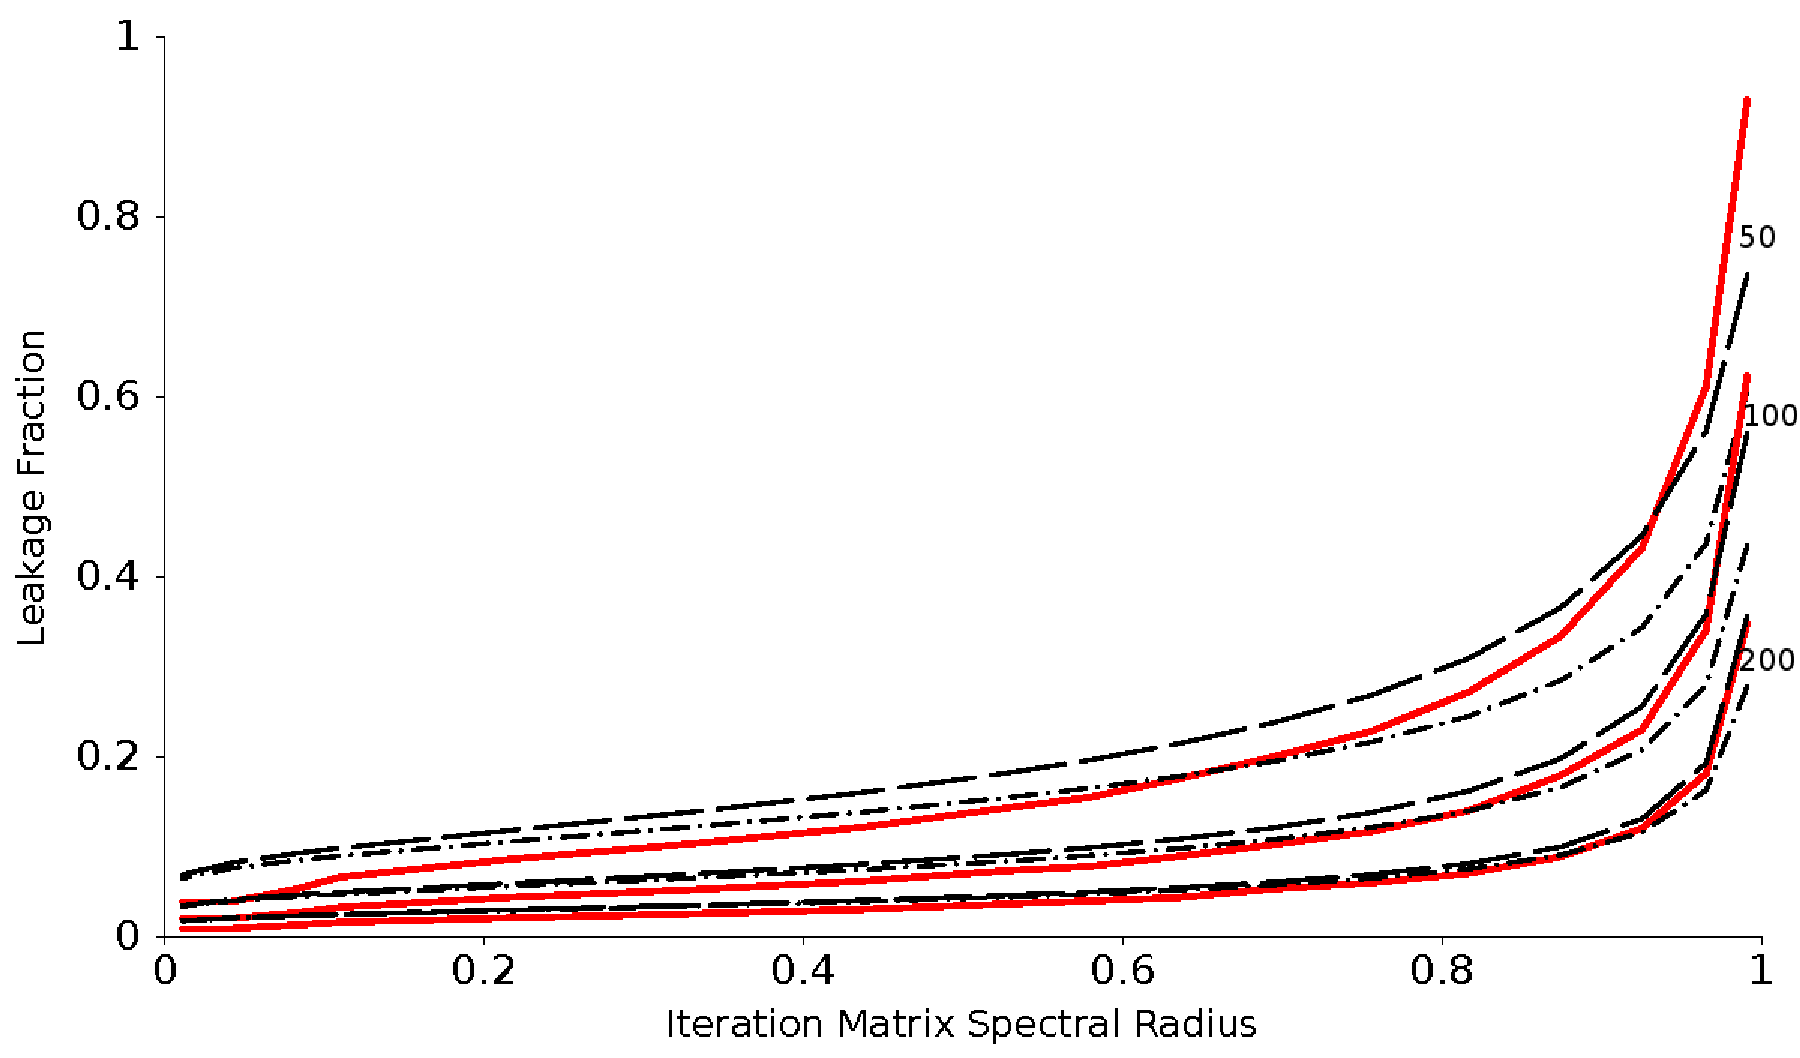
\includegraphics[width=4.75in,clip]{chapters/parallel_mc/leakage_variation_2.pdf}
    \end{center}
    \caption{\textbf{Measured and analytic domain leakage as a
        function of the iteration matrix spectral radius.} \textit{To
        test the behavior with respect to domain size, $n_i=50$,
        $n_i=100$,and $n_i=200$ were used. The red data was computed
        numerically by a domain-decomposed adjoint Neumann-Ulam
        implementation, the black dashed data was generated by
        Eq~(\ref{eq:mean_chord_domain_leakage}) using the mean-chord
        approximation, and the dashed-dotted black data was generated
        by Eq~(\ref{eq:wigner_domain_leakage}) using the Wigner
        rational approximation.}}
    \label{fig:measured_leakage}
  \end{spacing}
\end{figure}
Again, we note good qualitative agreement between the measured and
analytic quantities but we begin to see the limits of the leakage
approximations. 

To compare the quality of the two approximations, the absolute
difference between the computed leakage fraction and that generated by
the Wigner rational and mean chord approximations is plotted in
Figure~\ref{fig:leakage_error} for all domain sizes tested.
\begin{figure}[t!]
  \begin{spacing}{1.0}
    \begin{center}
      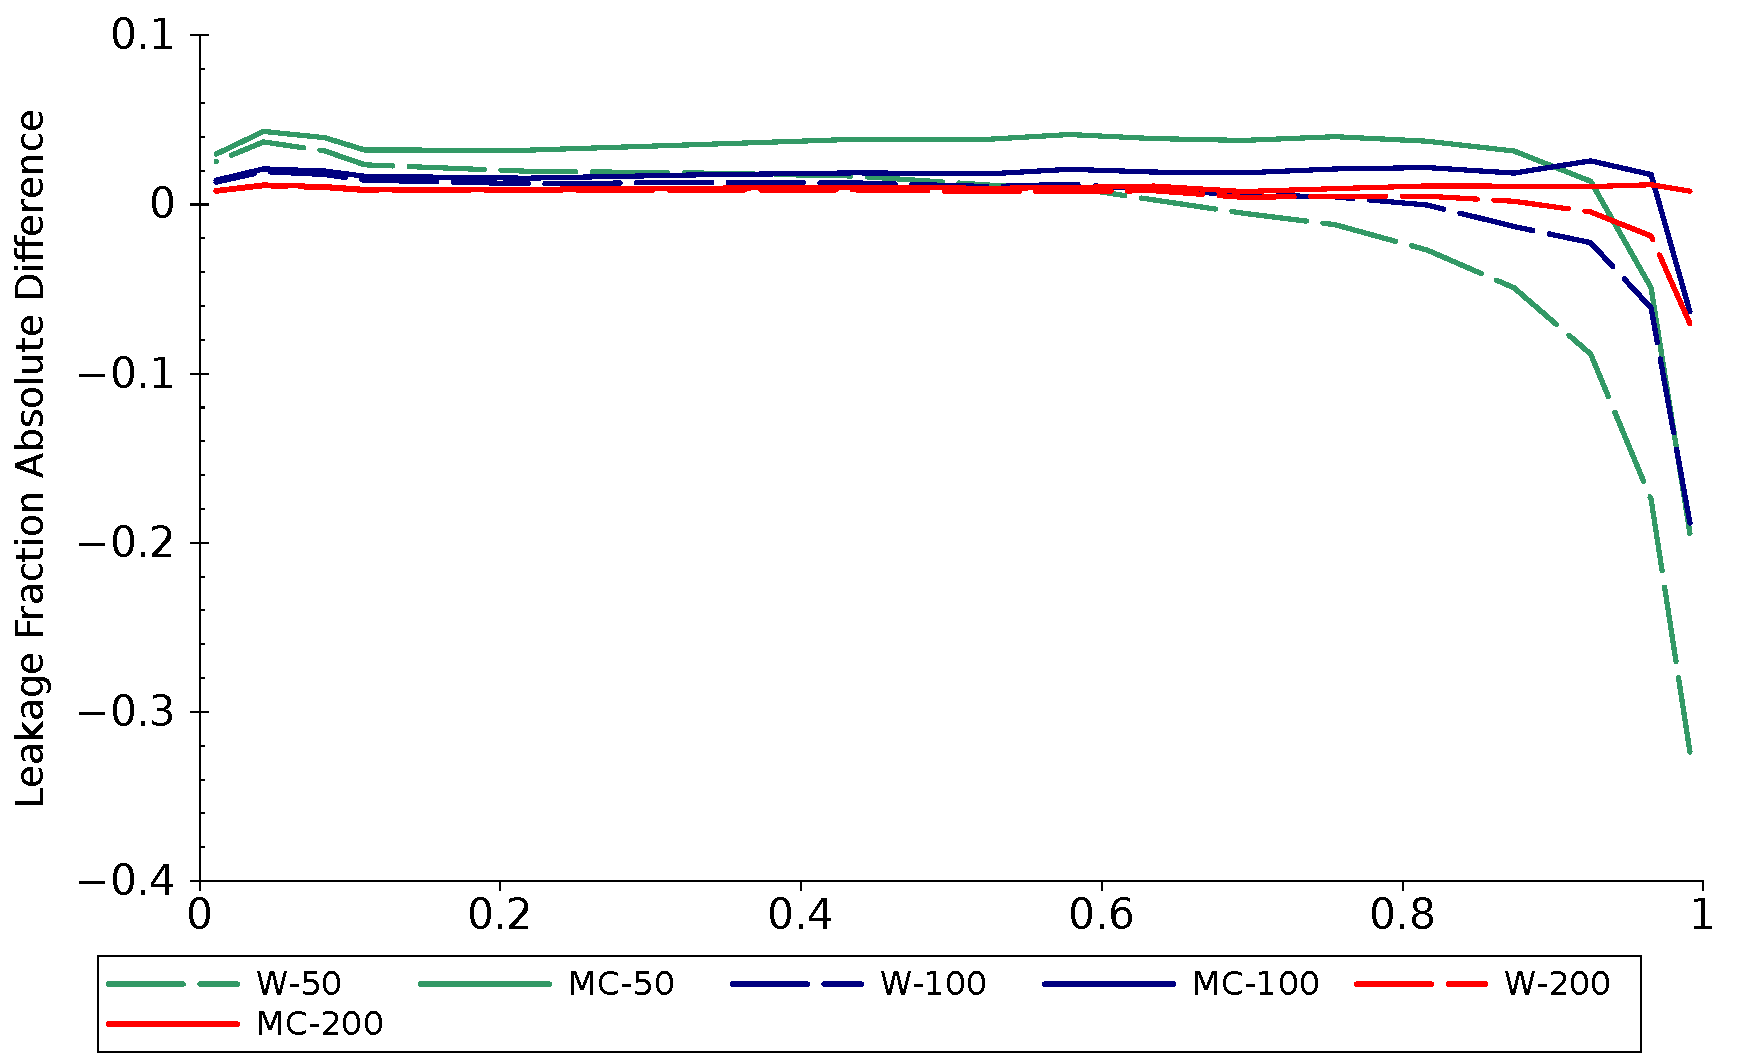
\includegraphics[width=4.75in,clip]{chapters/parallel_mc/leakage_error_2.pdf}
    \end{center}
    \caption{\textbf{Measured and analytic domain leakage absolute
        difference as a function of the iteration matrix spectral radius.}
      \textit{To test the behavior with respect to domain size,
        $n_i=50$ (green), $n_i=100$ (blue), and $n_i=200$ (red) were
        used. The dashed lines represent the difference using the Wigner
        rational approximation while the solid lines represent the
        difference using the mean-chord approximation.}}
    \label{fig:leakage_error}
  \end{spacing}
\end{figure}
From these difference results, the mean chord approximation is shown to
have a lower difference for ill-conditioned systems as compared to the
Wigner approximation while the Wigner approximation produces less
difference for more well-conditioned systems. We also note that for the
optically thick domains, the difference is likely corresponded to that
observed in Figure~\ref{fig:measured_length} for the $k$ parameter
while the large relative difference in $k$ for optically thin domains does
not affect the approximation significantly. In general, the mean chord
approximation is a better choice to estimate the leakage fraction in a
domain from the adjoint Neumann-Ulam method and except for a single
data point with $n_i=50$, the mean chord approximation yielded leakage
fractions within 0.05 of the measured results. As the domain becomes
more optically thick (with both increasing $n_i$ and decreasing
$\rho(\ve{H})$), the approximations are more accurate.

%%---------------------------------------------------------------------------%%
\section{Domain Decomposed Neumann-Ulam Algorithm\ }
\label{sec:asynchronous_algorithm}
In the context of radiation transport, in 2009 Brunner and colleagues
provided a fully asynchronous domain decomposed parallel algorithm as
implemented in production implicit Monte Carlo codes
\cite{brunner_efficient_2009}. We will adapt their algorithm and
directly apply it to a parallel formulation of the Neumann-Ulam
method. Direct analogs can be derived from their works by noting that
the primary difference between solving a linear transport system with
Monte Carlo methods and traditional fixed source Monte Carlo transport
problems is the content of the Markov chains that are generated. 

The transitions represented by these chains are bound by probabilities
and weights and are initiated by the sampling of a discrete source. In
the context of transport problems, those transitions represent events
such as particle scattering and absorption with probabilities that are
determined by physical data in the form of cross sections. For
stochastic matrix inversion, those transitions represent moving
between the equations of the linear system (and therefore the
components of phase space which they represent) and their
probabilities are defined by the coefficients of those
equations. Ultimately, we tally the contributions to generate
expectation values in the desired states as we progress through the
chains. Therefore, parallel methods for Monte Carlo radiation
transport can be abstracted and we can use those concepts that apply
to matrix inversion methods as an initial means of developing a
parallel Neumann-Ulam-type solver.

In this section Brunner and Brantley's fully asynchronous algorithm,
which was effectively implemented verbatim for this work, is presented
along with its application to the Neumann-Ulam method. For
considerably more detail, the algorithm presented can be found in
\cite{brunner_efficient_2009}. In their work they identify two data
sets that are required to be communicated: the sharing of particles
that are transported from one domain to another and therefore from one
processor to another and a global communication that signals if
particle transport has been completed on all processors. Both of these
communication sequences will be addressed at a high level along with
how the Monte Carlo data structures they require are constructed in
parallel.

\subsection{Parallel Transport Domain and Source }
\label{subsec:domain_generation}
To utilize a parallel transport algorithm, we must generate the
required data with the correct parallel decomposition. For the
Neumann-Ulam method, the transport domain consists of all states in
the system that are local, and the probabilities and weights for all
state transitions possible in the local domain. At the core of this
representation is the Neumann-Ulam decomposition of the linear
operator as given by Eq~\ref{eq:neumann_ulam_decomposition}. Given an
input decomposition for the linear operator, by definition the
Neumann-Ulam decomposition will have the same parallel
decomposition. In addition, any modification made to the linear
operator through preconditioning or relaxation parameters will also
modify the Neumann-Ulam decomposition. All possible transitions are
described by the local graph of the sparse input matrix. In addition,
any left preconditioning or relaxation parameters will modify the
right hand side of the linear system and therefore the fixed source in
the Monte Carlo calculation. This source vector will have the same
parallel decomposition as the input matrix and therefore all of the
birth states for the histories will exist for at least a single
transition event within the local domain.

Compared to the serial construction of the Neumann-Ulam decomposition,
data for all states that is required to be on process must be
collected in parallel. For the pure domain decomposition case, given
an input parallel decomposition for the Neumann-Ulam decomposition,
for all local states $m$ we require access to $P_{mn}$ and $W_{mn}$
(or $P^T_{mn}$ and $W^T_{mn}$) for the adjoint method for all possible
states $n$. Given by Figure~\ref{fig:diffusion_graph}, consider the
adjacency graph of a single state in the neutron diffusion matrix for
the model problem presented in Appendix~\ref{chap:diffusion_problem}.
\begin{figure}[t!]
  \begin{center}
    \scalebox{1.5}{ \input{chapters/parallel_mc/stencil_graph.pdftex_t} }
  \end{center}
  \caption{\textbf{Neutron diffusion equation state adjacency graph.}
    \textit{The structure of the graph comes from the discretization
      of the Laplacian operator describing the diffusion
      physics. Adjacent boundary states are collected by traversing
      the graph one step for all local boundary states and collecting
      the equations for those states that are not local. For a given
      transition in the random walk for the diffusion problem, a
      history at mesh point $(i,j)$ may transition to all adjacent
      mesh points including itself, corresponding to a global state
      transition from $m$ to $n$ in the linear system.}}
  \label{fig:diffusion_graph}
\end{figure}

In this example, we currently reside in state $m$ of the system,
directly correlating to physical location $(i,j)$ in the mesh (the
center node). The discretization stencil of the diffusion problem
dictates the structure of this graph and the states to which a history
may transition. If we play the Monte Carlo game to move to a new state
$n$, then we may move to any of the nodes in this graph, including the
node at which we started. If grid point $(i,j)$ in this example is on
the right of the local domain boundary and we transition to the right
to state $n$ corresponding to mesh point $(i+1,j)$, we are now in a
state that is owned by the adjacent domain. We must then gather the
data in the Neumann-Ulam decomposition from the neighboring process
that owns grid point $(i+1,j)$. Doing this provides us with the data
required by the estimators permitting $P_{mn}$ and $W_{mn}$ to be
computed locally for this particular boundary transition. In addition,
we also collect the identification number for the process that owns
this state such that we have an address to send all histories that
leave the local domain boundary for this state. For the parallel
source, these adjacent states are not required as histories may only
be born in states in the local domain. Once the local Neumann-Ulam
decomposition has been generated with the proper data collected from
adjacent domains, Monte Carlo transport may proceed in parallel.

\subsection{Domain Decomposed Algorithm}
\label{subsec:parallel_mc_algorithm}

Here we present in detail Brunner and Brantley's 2009 algorithm in
detail and discuss how it is adapted to parallelize the Neumann Ulam
method. Presented in Algorithm~\ref{alg:parallel_mc_algorithm}, the
top level sequence performs the task of managing history transport
through the local domain, communication of histories to adjacent
domains, and the completion of transport. For each of these specific
tasks, additional algorithms, shown in bold in
Algorithm~\ref{alg:parallel_mc_algorithm}
(e.g. \textbf{LocalHistoryTransport()}), are presented for additional
detail in the same manner as Brunner and Brantley.

\begin{algorithm}[h!]
  \caption{Parallel Neumann-Ulam Algorithm}
  \label{alg:parallel_mc_algorithm}
  \begin{algorithmic}[1]
    \State get list of neighbor processors 
    \Comment{Each neighbor owns an adjacent subdomain}
    \ForAll{neighbors}
    \State post nonblocking receive for maximum history buffer size
    \State allocate history buffer
    \EndFor
    \State \textit{historiesCompleted} = 0
    \Comment{local+child finished histories}
    \State \textit{localProcessed} = 0
    \Comment{local trajectories computed (not necessarily finished)}
    \State calculate parent and children processor ID numbers in
    binary tree
    \ForAll{child processes}
    \State post nonblocking receive for \textit{historiesCompleted} tally
    \EndFor
    \State post nonblocking receive for stop message from parent
    \While{stop flag not set}
    \If{any local histories in source or stack}
    \State \textbf{LocalHistoryTransport()}
    \State ++\textit{localProcessed}
    \EndIf
    \If{message check period == \textit{localProcessed} || no local histories}
    \State \textbf{ProcessMessages()}
    \State \textit{localProcessed} = 0
    \EndIf
    \If{no local histories}
    \State \textbf{ControlTermination()}
    \EndIf
    \EndWhile
    \State cancel outstanding nonblocking requests
    \State free all history buffers
  \end{algorithmic}
\end{algorithm}

Successful execution of this algorithm requires construction of the
parallel Neumann-Ulam decomposition as described in the preceding
section. This data is used to begin
Algorithm~\ref{alg:parallel_mc_algorithm} where lines 1-5 use the
collected list of neighboring processors generated while building the
Neumann-Ulam decomposition to setup the set of asynchronous messages
required for domain-to-domain communication. Again, consider this
communication pattern for the 9 subdomain example given by
Figure~\ref{fig:nearest_neighbor_comm}. In this pattern, each boundary
domain has two neighbors and the center domain four neighbors with
which they will communicate parallel histories and this communication
goes both ways as represented by the adjacent arrows in the
figure. For each set of neighbors, a non-blocking send and receive is
required with data buffers allocated with a user-defined size prepared
for incoming and outgoing histories. This nonblocking structure is
critical to the performance of the algorithm in that it permits local
history transport to continue while new histories to transport are
being collected in the buffers. When a given process is ready to do
more work, it can check these data buffers for incoming histories
requiring further transport. In this way there is a maximum amount of
overlap between communication and transport of histories.

\begin{figure}[t!]
  \begin{center}
    \scalebox{1.5}{ \input{chapters/parallel_mc/domain_to_domain.pdftex_t} }
  \end{center}
  \caption{\textbf{Nearest neighbor history communication sequence.}
    \textit{Each subdomain in the system has a set of nearest
      neighbors determined by the parallel adjacency graph of the
      input matrix. The subdomains are indexed by an integer.}}
  \label{fig:nearest_neighbor_comm}
\end{figure}

Once the nearest-neighbor communication sequence has been prepared,
the completion of transport sequence is readied in lines 6 and 8-12 in
Algorithm~\ref{alg:parallel_mc_algorithm}. In these lines we are
setting up an asynchronous binary communication tree as presented for
the same 9 subdomain example in Figure~\ref{fig:binary_comm_tree}. In
this communication pattern, each process has one parent process
(except for the MASTER process 0) to which it will nonblocking send
the number of histories that terminated their transport procedure by
weight cutoff in the local domain. Equivalently, each process has up
to two child processes from which it will receive their completed
number of histories with a nonblocking receive operation. Setting up a
tree in this manner lets the completed history tally
(\textit{historiesCompleted} in the algorithm) be updated
incrementally and funneled to the root process. Because we are
solving fixed source problems with the Neumann-Ulam algorithm without
any type of variance reduction that may generate more histories that
we started with, once the root process completion sum tallies to the
number of histories in the source, transport is complete. Once this
occurs, the root process nonblocking sends a process to its children
and each process nonblocking receives a stop message from its parent
as shown in Figure~\ref{fig:binary_comm_tree}. The stop message is
then propagated up the tree in the same manner.

\begin{figure}[t!]
  \begin{center}
    \scalebox{1.25}{
      \input{chapters/parallel_mc/binary_comm_tree.pdftex_t} }
    \caption{\textbf{Binary communication tree for coordinating the
        end of a parallel Neumann-Ulam solve.} \textit{Each child
        process reports to its parents how many histories completed
        within its domain. When the root process sums all complete
        histories, it forwards the stop signal to its children which
        in turn forward the message up the tree. The subdomains are
        indexed by an integer.}}
  \end{center}
  \label{fig:binary_comm_tree}
\end{figure}

With these communication structures prepared, we can now enter the
main transport loop at line 13 of
Algorithm~\ref{alg:parallel_mc_algorithm}. In this loop, a set of
mutually exclusive tasks enabled by the fully asynchronous
communication patterns are executed until the stop signal is received
from the parent process in the binary tree. In this case, mutually
exclusivity permits all local operations to occur independently of
other processes in the system and their current state. For each
process, there are two data structures from which histories may be
obtained for the transport procedure. The first is the local source
and the second is a LIFO (last in first out) stack of histories
transported to the local domain from the adjacent domain. In lines
14-17, if histories exist in either of these data structures, then
they are transported through the local domain using
Algorithm~\ref{alg:local_history_transport}. If the history is
terminated by weight cutoff the \textit{historiesCompleted} tally is
updated. If it hits the boundary of the domain it is added to the
outgoing history buffer for the neighboring domain and if the buffer
is full, it is sent to the neighboring domain with a nonblocking
operation and the memory associated with that buffer reallocated. In
all instances that Algorithm~\ref{alg:local_history_transport} is
executed, \textit{localProcessed} is incremented to account for
histories that have been processed locally.

\begin{algorithm}[h!]
  \caption{\textbf{LocalHistoryTransport()}}
  \label{alg:local_history_transport}
  \begin{algorithmic}[1]
    \State transport history through the domain until termination
    \If{history is in neighbor boundary state}
    \State add history to neighbor buffer
    \If{neighbor buffer is full}
    \State nonblocking send history buffer to neighbor
    \State allocate new history buffer for neighbor
    \EndIf
    \Else
    \If{history terminated by weight cutoff}
    \State post-process history
    \State ++\textit{historiesCompleted}
    \EndIf
    \EndIf
  \end{algorithmic}
\end{algorithm}

Continuing in the transport loop, if there are no local histories to
transport or the \textit{localProcessed} count has reached some
user-defined check frequency, lines 18-21 in
Algorithm~\ref{alg:local_history_transport} check for more histories
to transport in the incoming data buffers by calling
Algorithm~\ref{alg:process_messages}. For each neighboring domain in
the problem, if there are histories in those data buffers then they
are added to the stack from processing and the nonblocking receive
operation re-instantiated. In addition, the terminated histories count
is updated with those values received from the child processes.

\begin{algorithm}[h!]
  \caption{\textbf{ProcessMessages()}}
  \label{alg:process_messages}
  \begin{algorithmic}[1]
    \ForAll{received history buffers from neighbor}
    \State unpack number of histories in buffer
    \State add the histories to the running stack
    \State repost nonblocking receive with neighbor
    \EndFor
    \ForAll{\textit{historiesCompleted} messages from children}
    \State \textit{historiesCompleted} += message value
    \State repost nonblocking receive with child
    \EndFor
  \end{algorithmic}
\end{algorithm}

Finally, the transport loop finishes in lines 22-24 of
Algorithm~\ref{alg:local_history_transport} by calling
Algorithm~\ref{alg:control_termination} if there are no local
histories to transport in the stack or the source. In
Algorithm~\ref{alg:control_termination}, we continue to forward the
terminated history tally down to the parent in the binary tree and
send all history buffers to our neighbors, even if they are not
full. If Algorithm~\ref{alg:control_termination} is called by the
MASTER process, it checks for completion of the problem and if it is
complete, forwards to stop flag onto its children as in
Figure~\ref{fig:binary_comm_tree}. If the process is not the MASTER,
then we check for a stop signal from the parent and forward to the
child processes if transport is complete.

\begin{algorithm}[h!]
  \caption{\textbf{ControlTermination()}}
  \label{alg:control_termination}
  \begin{algorithmic}[1]
    \State nonblocking send an partially full history buffers
    \ForAll{\textit{historiesCompleted} messages from children}
    \State \textit{historiesCompleted} += message \textit{historiesCompleted}
    \State repost nonblocking receive with child
    \EndFor
    \If{MASTER processor}
    \If{\textit{historiesCompleted} == global \# of source histories}
    \State set stop flag
    \ForAll{children}
    \State nonblocking send stop message to child
    \EndFor
    \EndIf
    \Else
    \State nonblocking send \textit{historiesCompleted} to parent
    \State \textit{historiesCompleted} = 0
    \State check for stop signal from parent
    \If{stop signal from parent}
    \ForAll{children}
    \State nonblocking send stop message to child
    \EndFor
    \EndIf
    \EndIf
  \end{algorithmic}
\end{algorithm}

In this manner the transport loop continues until all process have
received the stop signal from their parents. Older versions of this
algorithm, particularly some of those presented in
\cite{brunner_comparison_2006}, use a master/slave approach as given
by Figure~\ref{fig:master_comm_tree} for the completion of a transport
stage instead of the binary tree scheme. In this approach, the root
process still manages the final summation of the completion tally, it
directly receives completed tally results from all other processes in
the problem instead of from just its children. Although this
implementation is potentially simpler to understand than the binary
tree approach, the authors of \cite{brunner_comparison_2006} observed
that this type of termination pattern, even when implemented in a
fully asynchronous manner, was a major scalability bottleneck. This
bottleneck is due to the fact that the master process falls behind the
others, creating a load imbalance even with the addition of a few
integer addition operations. We will explicitly demonstrate in scaling
studies how this bottleneck also occurs within a Neumann-Ulam
implementation of this algorithm thus requiring the implementation of
a binary communication tree.

\begin{figure}[t!]
  \begin{center}
    \scalebox{0.75}{
      \input{chapters/parallel_mc/master_comm_tree.pdftex_t} }
    \caption{\textbf{Master/slave scheme for coordinating the end of a
        parallel Neumann-Ulam solve.} \textit{Each slave process
        reports to the master how many histories completed within its
        domain. When the master process sums all complete histories,
        it sends the stop signal to all slave processes. The
        subdomains are indexed by an integer.}}
  \end{center}
  \label{fig:master_comm_tree}
\end{figure}

There is an additional advantage to Brunner and Brantley's work that
although not immediately applicable to this work has the potential to
provide value in the future. In addition to a robust fully
asynchronous communication pattern, this algorithm may also be modified
to account for situations where the total number of histories in a
given stage are not known before starting transport. From a physics
perspective, we might expect this for situations where perhaps an
(n,2n) interaction occurs in a neutronics problem. In this case, the
algorithm is modified to account for both histories terminated and
created and several mechanisms are introduced to determine completion
of the transport stage. For future variations of this work, certain
variance reduction techniques which create histories, such as
splitting, have the potential to be successfully employed as a means
of accelerating the time to solution for a given problem using
MCSA. The parallel Neumann-Ulam algorithm presented here may be
adapted to account for these additional techniques.

%%---------------------------------------------------------------------------%%
\section{Multiple-Set Overlapping-Domain Algorithm\ }
\label{subsec:msod}
Although the implementation presented in the previous section was
observed by Brunner and Brantley to be robust and allowed for scaling
to large numbers of processors, performance issues were still noted
with parallel efficiency improvements needed in both the weak and
strong scaling cases for unbalanced problems. These results led them
to conclude that a combination of domain decomposition and domain
replication could be used to solve some of these issues. In 2010,
Wagner and colleagues developed the \textit{multiple-set
  overlapping-domain} (MSOD) decomposition for parallel Monte Carlo
applications for full-core light water reactor analysis
\cite{wagner_hybrid_2010}. In their work, an extension of Brunner's,
their scheme employed similar parallel algorithms for particle
transport but a certain amount of overlap between adjacent domains was
used to decrease the number of particles leaving the local domain. In
addition, Wagner utilized a level of replication of the domain such
that the domain was only decomposed on $O(100)$ processors and if
replicated $O(1,000)$ times potentially achieves efficient simulation
on $O(100,000)$ processors, thus providing both spatial and particle
parallelism.

Each collection of processors that constitutes a representation of the
entire domain is referred to as a set, and within a set overlap occurs
among its sub-domains. The original motivation was to decompose the
domain in a way that it remained in a physical cabinet in a large
distributed machine, thus reducing latency costs during
communication. A multiple set scheme is also motivated by the fact
that communication during particle transport only occurs within a set,
limiting communications during the transport procedure to a group of
$O(100)$ processors, a number that was shown to have excellent
parallel efficiencies in Brunner's work and therefore will scale well
in this algorithm. The overlapping domains within each set also
demonstrated reduced communication costs. On each processor, the
source is sampled in the local domain that would exist if no overlap
was used while tallies can be made over the entire overlapping domain.

To demonstrate this, consider the example adapted from Mervin's work
with Wagner and others in the same area \cite{mervin_variance_2012}
and presented in Figure~\ref{fig:msod_example}.
\begin{figure}[t!]
  \begin{center}
    \scalebox{1.5}{
      \input{chapters/parallel_mc/msod_example.pdftex_t} }
  \end{center}
  \caption{\textbf{Overlapping domain example illustrating how domain
      overlap can reduce communication costs.}
    \textit{All particles start in the blue region of interest. The
      dashed line represents 0.5 domain overlap between domains.}}
  \label{fig:msod_example}
\end{figure}
In this example, 3 particle histories are presented emanating from the
blue region of interest. Starting with particle A, if no domain
overlap is used then the only the blue domain exists on the starting
processor. Particle A is then transported through 3 other domains
before the history ends, therefore requiring three communications to
occur in Brunner's algorithm. If a 0.5 domain overlap is permitted as
shown by the dashed line, then the starting process owns enough of the
domain such that no communications must occur in order to complete the
particle A transport process. Using 0.5 domain overlap also easily
eliminates cases such as that represented by the path of particle
C. In this case, particle C is scattering between two adjacent
domains, incurring a large latency cost for a single
particle. Finally, with particle B we observe that 0.5 domain overlap
will still not eliminate all communications. However, if 1 domain
overlap were used, the entire geometry shown in
Figure~\ref{fig:msod_example} would be contained on the source
processor and therefore transport of all 3 particles without
communication would occur.

Wagner and colleagues used this methodology for a 2-dimensional
calculation of a pressurized water reactor core and varied the domain
overlap from 0 to 3 domain overlap (a $7 \times 7$ box in the context
of our example) where a domain contained an entire fuel assembly. For
the fully domain decomposed case, they observed that 76.12\% of all
source particles leave the domain. At 1.5 domain overlap, the
percentage of source particles born in the center assembly leaving the
processor domain dropped to 1.05\% and even further for 0.02\% for the
3 domain overlap. Based on their results, we hypothesize that the
overlap approach coupled with the multiple sets paradigm that will
enhance the scalability of the pure domain-decomposition algorithm for
Neumann-Ulam presented in the previous section.

\subsection{Generating the MSOD Decomposition }
\label{subsec:msod_generation}
In \S~\ref{subsec:domain_generation} we discussed how we generated the
parallel transport domain from the Neumann-Ulam decomposition of a
domain decomposed linear operator. We can readily adapt those data
structures to account for the extra information required by an
implementation of the MSOD algorithm. First, we consider the
generation of overlap. Conveniently, this is identical to the
neighboring states discovery problem discussed in conjunction with
Figure~\ref{fig:diffusion_graph}. To generate the boundary for the
local transport domain, we needed to gather all data from the
immediately adjacent states in the system that did not already exist
in the local domain. We solved this problem by traversing the graph
of the matrix for each of the boundary states and determining which
processes owned those adjacent states. 

To generate overlap, we use the identical algorithm but in this case
we perform as many graph level traversals as the specified amount of
overlap. For example, consider the analytic relations derived in
\S~\ref{sec:analytic_framework} for the length of random walks in a
Neumann-Ulam method and the amount of leakage from a domain
considering a neutron diffusion problem. From these relations we might
determine that, for our particular problem, if we can grow the domain
by 10 additional discrete state transitions, we can reduce the number
of histories that must be communicated by a significant fraction. We
determine the information we must gather from neighboring domains to
build the overlap by traversing the graph of the matrix outward from
the boundary 10 levels. At each step, we find the data in the adjacent
domain that we require and make that data local, incrementing the size
of the overlap. Once the overlap has been gathered, one extra graph
traversal on the boundary states is performed to get the new
neighboring states and their owning processes.

Once overlap has been generated, the transport domain for a single set
is complete. However, if multiple sets are to be used, an additional
set of parallel procedures is required to generate the necessary data
structures. Figure~\ref{fig:msod_construction} gives a schematic
representation of the MSOD construction process using 4 sets. For a
problem where $P$ parallel processors are available and $S$ sets are
to be used, each set is allocated $P/S$ processors for computation. On
the first $P/S$ processors, the linear problem is generated. From the
linear problem, the linear operator is used to construct the transport
domain, the solution vector used to construct the tallies, and the
forcing term vector used to construct the fixed source. Once these
Monte Carlo data structures have been generated, they are broadcast to
the remaining sets in the problem as shown in
Figure~\ref{fig:msod_construction} such that we have $S$ replications
of the Monte Carlo problem for a single instance of the original
linear problem.

\begin{figure}[t!]
  \begin{center}
    \scalebox{0.6}{ \input{chapters/parallel_mc/msod_construction.pdftex_t} }
  \end{center}
  \caption{\textbf{MSOD construction for 4 sets with overlap.}
    \textit{The linear system is used to construct the Monte Carlo
      transport domain on the primary set. The Monte Carlo data
      structures are then broadcast among the blocks to all sets in
      the system.}}
  \label{fig:msod_construction}
\end{figure}

\clearpage

\subsection{MSOD Neumann Ulam Algorithm }
\label{subsec:msod_algorithm}

With the ability to generate the transport domain within an MSOD
decomposition as well as the source and tally structures, we can now
define how to perform a Neumann-Ulam solve using MSOD. Given by
Algorithm~\ref{alg:msod_transport}, we begin by constructing the Monte
Carlo data structures for each set including the transport domain, the
source, and the tallies. Next, in line 4 we perform the asynchronous
transport algorithm presented in \S~\ref{sec:asynchronous_algorithm}
for each of the individual sets. Adding overlap to
Algorithm~\ref{alg:parallel_mc_algorithm} in this case simply modifies
the set of local states and the set of neighboring states to
additional states gathered during overlap generation.

\begin{algorithm}[h!]
  \caption{\textbf{MSOD Transport Sequence}}
  \label{alg:msod_transport}
  \begin{algorithmic}[1]
    \State build MSOD domain
    \State build Monte Carlo source
    \State build Monte Carlo tally
    \State perform parallel Neumann-Ulam transport in each set
    \State combine set tallies
    \State combine block tallies
  \end{algorithmic}
\end{algorithm}

Once Monte Carlo transport is complete complete, the tallies for each
individual computation must be gathered to the original set in order
to build the correction vector within an MCSA sequence. To do this, we
perform two parallel vector operations. First, overlap not only
creates additional states in the local transport domain but also
additional states in the local tally vector such that any events that
occur in the local domain may be tallied in a local vector. Because of
this, the tally vector in a single set will share local states with
other domains and a parallel sum reduction operation is required to
transform the tally into the original Neumann-Ulam parallel
decomposition. Second, the tallies in individual sets must be combined
and applied to the primary set in the problem that shares the
processor space with the original linear problem. For this operation,
we employ the concept of blocks as a subdivision of parallel space
complementary to the concept of sets.

Consider the schematic representation of the final parallel reduction
presented in Figure~\ref{fig:msod_tally_reduction}. For this
operation, the tally vectors in each set must be summed together and
applied to the primary set. As each set is an exact replica of the
others, the parallel decomposition of the tally vector is the same
within all sets. We can take advantage of this by building a processor
space that encapsulates each identical domain in each set. We can then
use this processor space for the reduction. For the schematic in
Figure~\ref{fig:msod_tally_reduction}, the upper-left domain in each
set creates a single block, giving 9 total blocks for this example
problem. The processor space that encapsulates each of the upper-left
domains is then used for the parallel reduction operation. This
reduction will happen in a mutually exclusive manner for each of the
blocks in the system. One benefit of this approach is that this
reduction occurs only over a subset of the processors in the problem,
providing better scalability than a reduction operation over all
processors in the problem.

\begin{figure}[t!]
  \begin{center}
    \scalebox{0.6}{ \input{chapters/parallel_mc/msod_tally.pdftex_t} }
  \end{center}
  \caption{\textbf{MSOD tally reduction over blocks.} \textit{The
      tally computed independently in each set is reduced across the
      blocks to the primary set. The linear system vector is updated
      on the primary set. In this example the tally vector in the
      block containing upper-left subdomains is combined. Identical
      reduction operations occur for all other blocks
      simultaneously.}}
  \label{fig:msod_tally_reduction}
\end{figure}

\clearpage

%%---------------------------------------------------------------------------%%
\section{Parallel MCSA\ }
\label{sec:parallel_mcsa}
With the parallel adjoint Neumann-Ulam solver implementation described
above, the parallel implementation of an MCSA iteration is
trivial. Recall the MCSA iteration procedure presented again here for
clarity:
\begin{subequations}
  \begin{gather}
    \label{eq:mcsa_r1}
    \ve{x}^{k+1/2} = \ve{x}^k + \ve{r}^k\:,\\
    \label{eq:mcsa_r2}
    \ve{r}^{k+1/2} = \ve{b} - \ve{A}\ve{x}^{k+1/2}\:,\\
    \label{eq:mcsa_r3}
    \ve{A}\delta\ve{x}^{k+1/2} = \ve{r}^{k+1/2}\:,\\
    \label{eq:mcsa_r4}
    \ve{x}^{k+1} = \ve{x}^{k+1/2} + \delta \ve{x}^{k+1/2}\:,\\
    \label{eq:mcsa_r5}
    \ve{r}^{k+1} = \ve{b} - \ve{A}\ve{x}^{k+1}\:.
  \end{gather}
\end{subequations}
In \S\ref{sec:parallel_krylov_methods} we discuss parallel matrix and
vector operations as utilized in conventional projection methods. We
utilize these here for the parallel MCSA implementation for the
computations required in Eqs~(\ref{eq:mcsa_r1}), (\ref{eq:mcsa_r2}),
(\ref{eq:mcsa_r4}), and (\ref{eq:mcsa_r5}). In the first step, a
parallel matrix-vector multiply is used to apply the split operator to
the previous iterate's solution. A parallel vector update is then
performed with the source vector to arrive at the initial iteration
guess. In the next step, the residual is computed by the same
operations where now the operator is applied to the solution guess
with a parallel matrix-vector multiply and then a parallel vector
update with the source vector is performed. Once the correction is
computed with a parallel adjoint Neumann-Ulam solve, this correction
is applied to the guess with a parallel vector update to get the new
iteration solution. Additionally, as given by
Eq~(\ref{eq:mcsa_stopping_criteria}), 2 parallel vector reductions
will be required to check the stopping criteria: one initially to
compute the infinity norm of the source vector, and another at every
iteration to compute the infinity norm of the residual vector.

To parallelize the solution of Eq~(\ref{eq:mcsa_r3}), we apply the
MSOD Neumann-Ulam algorithm presented in the previous section. The
problem is potentially replicated with overlap and the Monte Carlo
procedure returns a correction vector, $\delta \ve{x}$, with the same
parallel decomposition as the input linear problem. As was the case
for generating the replications required for a multiple set
implementation, the explicit matrix and vector operations required for
the rest of an MCSA iteration occur only on the subset of processors
containing the primary set. Only the Monte Carlo data structures exist
on the rest of the processors in the problem as replication of the
other operations does not generate any more information that could be
used to accelerate the time to solution.

\subsection{Parallel FANM Implementation}
\label{subsec:parallel_fanm}
Here we briefly comment on how a FANM method may be implemented in
parallel. A parallel FANM method relies on a basic set of parallel
matrix-vector operations outlined in
\S~\ref{sec:parallel_krylov_methods} as well as the global residual
and Jacobian assembly procedure described in
\S~\ref{subsec:automatic_differentiation}. Consider the FANM iteration
scheme in Algorithm~\ref{alg:fanm}. We must first assemble the linear
system in parallel through the element-wise function evaluations to
generate both the global Jacobian operator and the global residual
vector on the right hand side. Per Bartlett's work on automatic
differentiation, efficient and automated parallel mechanisms are
available to do this through a sequence of scatter/gather
operations. With these tools available for residual and Jacobian
generation, the remainder of the parallel procedure is simple. The
linear Newton correction system is solved using the parallel MCSA
method as described in the previous section and the Newton correction
applied to the previous iterate's solution through a parallel vector
update.

%%---------------------------------------------------------------------------%%
\section{Parallel MCSA Verification\ }
\label{sec:parallel_verification}
Before we consider the parallel performance of the MCSA algorithm, we
must first verify that the algorithm generates the correct solution in
parallel with respect to reference solutions provided by production
Krylov methods. To verify correctness, we use solutions to the neutron
diffusion system presented in
Appendix~\ref{chap:diffusion_problem}. As the reference computation,
serial results will be used from the conjugate gradient solver in
Belos, a linear solvers package in the Trilinos scientific computing
libraries \cite{heroux_overview_2005}. In identical fashion to the
verification for the $SP_N$ equations performed in
\S~\ref{sec:spn_mcsa_verification}, we will solve the neutron
diffusion problem in parallel using multiple cores on a desktop
machine. For each parallel solution, then the solution at each grid
point in the system will be compared to the solution at the same grid
point in the serial reference case with the minimum and maximum
absolute differences of these values reported.

GMRES and conjugate gradient solvers from the Belos package were used
on 4 cores as a means of both assuring the Krylov solvers produce the
same results on multiple cores and as a means of providing an
acceptable range of minimum and maximum values in the comparison. For
MCSA, a range of MSOD parameters will be used such that problems with
multiple sets and multiple blocks may be tested along with
overlap. For all MCSA calculations, a single history was used for
every DOF in the problem to compute the correction vector. For all
solvers, the flux was converged to a tolerance of \sn{1}{-8} and
therefore if the comparisons agree within this tolerance the solutions
will be deemed
correct. Table~\ref{tab:parallel_verification_parameters} gives the
parameters for the verification problem and
Table~\ref{tab:parallel_mcsa_verification} gives the results of the
calculations. Solver parameters used for MCSA are given in
Table~\ref{tab:parallel_mcsa_parameters}.

\begin{table}[h!]
  \begin{center}
    \begin{tabular}{lc}\hline\hline
      \multicolumn{1}{l}{Parameter}& 
      \multicolumn{1}{c}{Value}\\\hline
      $dx$ & 0.1 \\
      $dy$ & 0.1 \\
      $N_x$ & 400 \\
      $N_y$ & 400 \\
      $N$ & 160,000 \\
      $\Sigma_a$ & 5.0 \\
      $\Sigma_s$ & 1.0 \\
      Boundary Type & Vacuum \\
      Linear Solver Tolerance & \sn{1}{-8} \\
      %%
      \hline\hline
    \end{tabular}
  \end{center}
  \caption{\textbf{Parallel MCSA verification model problem parameters.}
    \textit{The neutron diffusion equation in 2 dimensions is used for
      the model problem.}}
  \label{tab:parallel_verification_parameters}
\end{table}

\begin{table}[h!]
  \begin{center}
    \begin{tabular}{lc}\hline\hline
      \multicolumn{1}{l}{Parameter}& 
      \multicolumn{1}{c}{Value}\\\hline
      Histories & 1 per DOF \\
      Weight Cutoff & \sn{1}{-2} \\
      Fixed Point Iteration & Richardson \\
      Estimator & Adjoint Collision \\
      %%
      \hline\hline
    \end{tabular}
  \end{center}
  \caption{\textbf{Parallel MCSA verification solver parameters.}
    \textit{No relaxation parameters or variance reduction techniques
      were used with MCSA.}}
  \label{tab:parallel_mcsa_parameters}
\end{table}

\begin{table}[h!]
  \begin{center}
    \begin{tabular}{lccccll}\hline\hline
      \multicolumn{1}{l}{Solver}& 
      \multicolumn{1}{c}{Blocks}& 
      \multicolumn{1}{c}{Sets}& 
      \multicolumn{1}{c}{Cores}& 
      \multicolumn{1}{c}{Overlap}& 
      \multicolumn{1}{l}{Min Difference}& 
      \multicolumn{1}{l}{Max Difference}\\\hline
      Conjugate Gradient & - & - & 4 & - & 0.0 & \sn{1.11022}{-16} \\
      GMRES & - & - & 4 & - & \sn{5.64215}{-13} & \sn{3.83348}{-9} \\
      MCSA & 2 & 1 & 2 & 0 & \sn{8.60423}{-16} & \sn{7.6806}{-9} \\
      MCSA & 3 & 1 & 3 & 0 & \sn{6.41154}{-15} & \sn{7.65397}{-9} \\
      MCSA & 4 & 1 & 4 & 0 & \sn{2.66454}{-15} & \sn{7.62623}{-9} \\
      MCSA & 2 & 2 & 4 & 0 & \sn{1.52656}{-15} & \sn{7.57108}{-9} \\
      MCSA & 1 & 4 & 4 & 0 & \sn{5.55112}{-16} & \sn{7.61631}{-9} \\
      MCSA & 8 & 1 & 8 & 0 & \sn{6.13398}{-15} & \sn{7.51744}{-9} \\
      MCSA & 4 & 2 & 8 & 0 & \sn{1.03251}{-14} & \sn{7.62601}{-9} \\
      MCSA & 2 & 4 & 8 & 0 & \sn{5.13478}{-15} & \sn{7.60777}{-9} \\
      MCSA & 1 & 8 & 8 & 0 & \sn{1.80411}{-15} & \sn{7.60651}{-9} \\
      MCSA & 2 & 1 & 2 & 5 & \sn{2.47025}{-15} & \sn{7.58882}{-9} \\
      MCSA & 3 & 1 & 3 & 5 & \sn{2.44249}{-15} & \sn{7.6326}{-9} \\
      MCSA & 4 & 1 & 4 & 5 & \sn{7.49401}{-16} & \sn{7.49014}{-9} \\
      MCSA & 2 & 2 & 4 & 5 & \sn{1.19349}{-15} & \sn{7.61814}{-9} \\
      MCSA & 1 & 4 & 4 & 5 & \sn{5.55112}{-16} & \sn{7.61631}{-9} \\
      MCSA & 8 & 1 & 8 & 5 & \sn{2.05391}{-15} & \sn{7.63955}{-9} \\
      MCSA & 4 & 2 & 8 & 5 & \sn{9.57567}{-15} & \sn{7.61313}{-9} \\
      MCSA & 2 & 4 & 8 & 5 & \sn{5.7454}{-15} & \sn{7.60767}{-9} \\
      MCSA & 1 & 8 & 8 & 5 & \sn{1.80411}{-15} & \sn{7.60651}{-9} \\
      MCSA & 2 & 1 & 2 & 10 & \sn{1.08247}{-15} & \sn{7.63231}{-9} \\
      MCSA & 3 & 1 & 3 & 10 & \sn{3.27516}{-15} & \sn{7.60211}{-9} \\
      MCSA & 4 & 1 & 4 & 10 & \sn{4.996}{-16} & \sn{7.64756}{-9} \\
      MCSA & 2 & 2 & 4 & 10 & \sn{4.13558}{-15} & \sn{7.60259}{-9} \\
      MCSA & 1 & 4 & 4 & 10 & \sn{5.55112}{-16} & \sn{7.61631}{-9} \\
      MCSA & 8 & 1 & 8 & 10 & \sn{9.71445}{-16} & \sn{7.58535}{-9} \\
      MCSA & 4 & 2 & 8 & 10 & \sn{7.77156}{-16} & \sn{7.65978}{-9} \\
      MCSA & 2 & 4 & 8 & 10 & \sn{4.16334}{-16} & \sn{7.63191}{-9} \\
      MCSA & 1 & 8 & 8 & 10 & \sn{1.80411}{-15} & \sn{7.60651}{-9} \\
      %%
      \hline\hline
    \end{tabular}
  \end{center}
  \caption{\textbf{Parallel MCSA verification results.}
    \textit{Difference values given are absolute values. The neutron
      diffusion equation in 2 dimensions is used for the model problem
      with the parameters given in
      Table~\ref{tab:parallel_verification_parameters}. A serial
      conjugate gradient calculation is used as the reference
      computation and neutron fluxes are compared
      element-wise. Parameters used for the MCSA solver are given in
      Table~\ref{tab:parallel_mcsa_parameters}. All solvers including
      the reference computation were converged to tolerance of
      \sn{1}{-8}.}}
  \label{tab:parallel_mcsa_verification}
\end{table}

From the data we see that for all solvers the parallel results agree
with the reference serial results within the solution tolerance for
all DOF in the system. In addition, we do not notice any systematic
differences in the results as a function of number of blocks, number
of sets, or amount of overlap. In addition, the parallel GMRES results
have maximum absolute differences of the same magnitude as all MCSA
results and a larger minimum absolute difference than all MCSA results
by three orders of magnitude. Based on these results, MCSA
parallelized with the MSOD algorithm, and in particular the
implementation used here, generates the correct results with respect
to the serial conjugate gradient reference computation.

\clearpage

%%---------------------------------------------------------------------------%%
\section{Leadership-Class Parallel Scaling Studies\ }
\label{sec:leadership_scaling_studies}
Using the parallel performance metrics presented in
Appendix~\ref{chap:parallel_metrics}, we will next measure performance
in various scaling studies using an implementation of the parallel
MCSA algorithm to assess its quality using the neutron diffusion
problem presented in Appendix~\ref{chap:diffusion_problem}. For these
scaling studies, large problems at high levels of concurrency will be
solved at a leadership-class computing facility. In this section, we
will outline the parallel machine on which the calculations were
performed and then present a series of numerical studies that identify
both strengths and weaknesses of the parallel algorithm. Both pure
domain decomposition and MSOD parallel performance will be explored
and compared to performance results for the same problems using a set
of production parallel Krylov solvers.

For the scaling results presented here, all parallel MCSA results were
computed using the Monte Carlo Linear Solvers\footnote{MCLS is an open
  source C++ library built on the Trilinos framework and can be
  downloaded at \url{https://github.com/sslattery/MCLS}} (MCLS)
library generated specifically for this work while the conjugate
gradient and GMRES Krylov solvers used are part of the Belos linear
solver package within the Trilinos framework
\cite{heroux_overview_2005}. In general, the Belos package produces
solutions to the neutron diffusion problem nearly two orders of
magnitude faster than the MCLS library for serial computations using
the conjugate gradient solver. Therefore, when we directly compare
these two codes, the MCLS parallel efficiencies will appear
artificially inflated relative to the Belos efficiencies due to the
fact that the MCLS ratio of work to communication will be much larger
than that for the Belos calculations. For every scaling study
presented, the calculations were performed 3 times with the average
values reported for wall time and those average values used for the
efficiency computations. In addition, it should be noted that in
practice, symmetric positive-definite problems like the neutron
diffusion problem solved here would never be solved using
GMRES. Instead, a method such as conjugate gradient would typically be
used due to the enhanced performance. We use GMRES here simply as a
means of providing an additional comparison for MCSA performance.

\subsection{Titan }
\label{subsec:titan}
All parallel scaling studies presented in this work were performed on
the Titan Cray XK7 machine at the Oak Ridge Leadership Computing
Facility located at Oak Ridge National Laboratory. Titan is a
heterogeneous architecture machine combining both CPU and GPU
components to achieve a theoretical peak performance of more than 20
petaflops. The technical specifications for Titan for only the CPU
portion of the machine are given in Table~\ref{tab:titan_hardware}.

\begin{table}[h!]
  \begin{center}
    \begin{tabular}{lc}\hline\hline
      Processor & 16 core AMD \\
      Nodes & 18,688 AMD Opterons \\
      Cores/Node & 16 \\
      Total Cores & 299,008 \\
      Memory/Node & 32 GB \\
      Memory/Core & 2 GB \\
      Interconnect & Gemini \\
      %%
      \hline\hline
    \end{tabular}
  \end{center}
  \caption{\textbf{Titan Cray XK7 hardware specifications.}
    \textit{Specifications presented for Titan in this table were
      gathered from the Oak Ridge Leadership Computing Facility at}
    \url{http://www.olcf.ornl.gov/computing-resources/titan-cray-xk7/}}
  \label{tab:titan_hardware}
\end{table}

For the scaling studies presented in this work, only the CPU
components of Titan specified in Table~\ref{tab:titan_hardware} were
utilized. This is due to the fact that the implementations of the
parallel MCSA algorithm in the MCLS library utilized code written only
with the Message Passing Interface (MPI) and therefore could not take
advantage of the GPU accelerators. Even considering just the CPU
portion of Titan, nearly 300,000 CPUs are available to test the
parallel performance of the MCSA algorithm at high levels of
concurrency.

For each parallel performance metric presented in the previous
section, a reference case is required to compute efficiencies for all
other cases. For smaller machines, often a serial computation can be
performed and used as the base case to get a true measure of speed-up
for a particular problem. For our scaling studies, we will always use
as a reference case a calculation which uses 16 cores, filling an
entire node of the machine. We fill an entire node so that we may
ignore the effects on scalability measures that arise from using only
a subset of cores in a node. Typically this results in a large drop in
efficiency from a serial computation to a calculation that fills the
entire node. Once a node is filled, adding subsequent nodes has less
of an effect on the scaling, providing a more stable region of
analysis.

\subsection{Communication Parameters}
\label{subsec:comm_parameters}

In our description of Brunner and Brantley's algorithm as applied to
the Neumann-Ulam method, we noted two free parameters that are
user-defined at runtime. The first is the static data buffer size for
communicating histories between neighboring domains and the second is
the frequency by which a domain checks for incoming information from
neighboring domain, both of which may potentially affect latency and
load balancing. Changing the static history buffer size parameter
affects the scalability of the algorithm in two ways. If the buffer
size is increased, the buffer takes longer to fill and is therefore
sent less frequently, potentially causing load balancing bottlenecks
where a neighboring domain is idle and waiting for more work to do but
is waiting for another domain to complete work. In addition, if the
buffer size is too large, the network may become saturated with these
very large data packets, slowing down performance. If the buffer size
is too small, too many history messages are sent, not providing enough
data for a neighboring process to work on to make up for the time
spent communicating. Considering the second parameter, when the
message check frequency period is increased, more histories are
processed locally before looking to do work elsewhere. If this value
becomes too large, incoming data buffers may not be cleared frequently
enough and cause decreased performance in the domain-to-domain
communications. If this value is too small, too much time is spent
looking for work instead of actually performing it.

To assess how these parameters affect the performance of the parallel
Monte Carlo algorithm on the Titan machine, a parameter study was
performed using the neutron diffusion problem on 64 cores (4
nodes). This problem had a reasonably well conditioned spectral radius
of 0.78 with a global problem size of \sn{1.6}{7} DOFs with one
stochastic history used per DOF in the MCSA Neumann-Ulam used to
compute the correction for the acceleration. Each parameter was varied
between 16 and 4096 and the time to solve the problem recorded. The
results of this study are presented in
Figure~\ref{fig:titan_comm_parameters}. Compared to the results of
Brunner and Brantley for the same type of study, we note qualitatively
similar results with the general observation that a larger history
buffer check period is better than a shorter one. The larger the check
period, the more on-process work is done before checking
messages. Second, there was not a significant variation observed in
the history buffer size parameter for a given check frequency.

\begin{figure}[t!]
  \begin{center}
    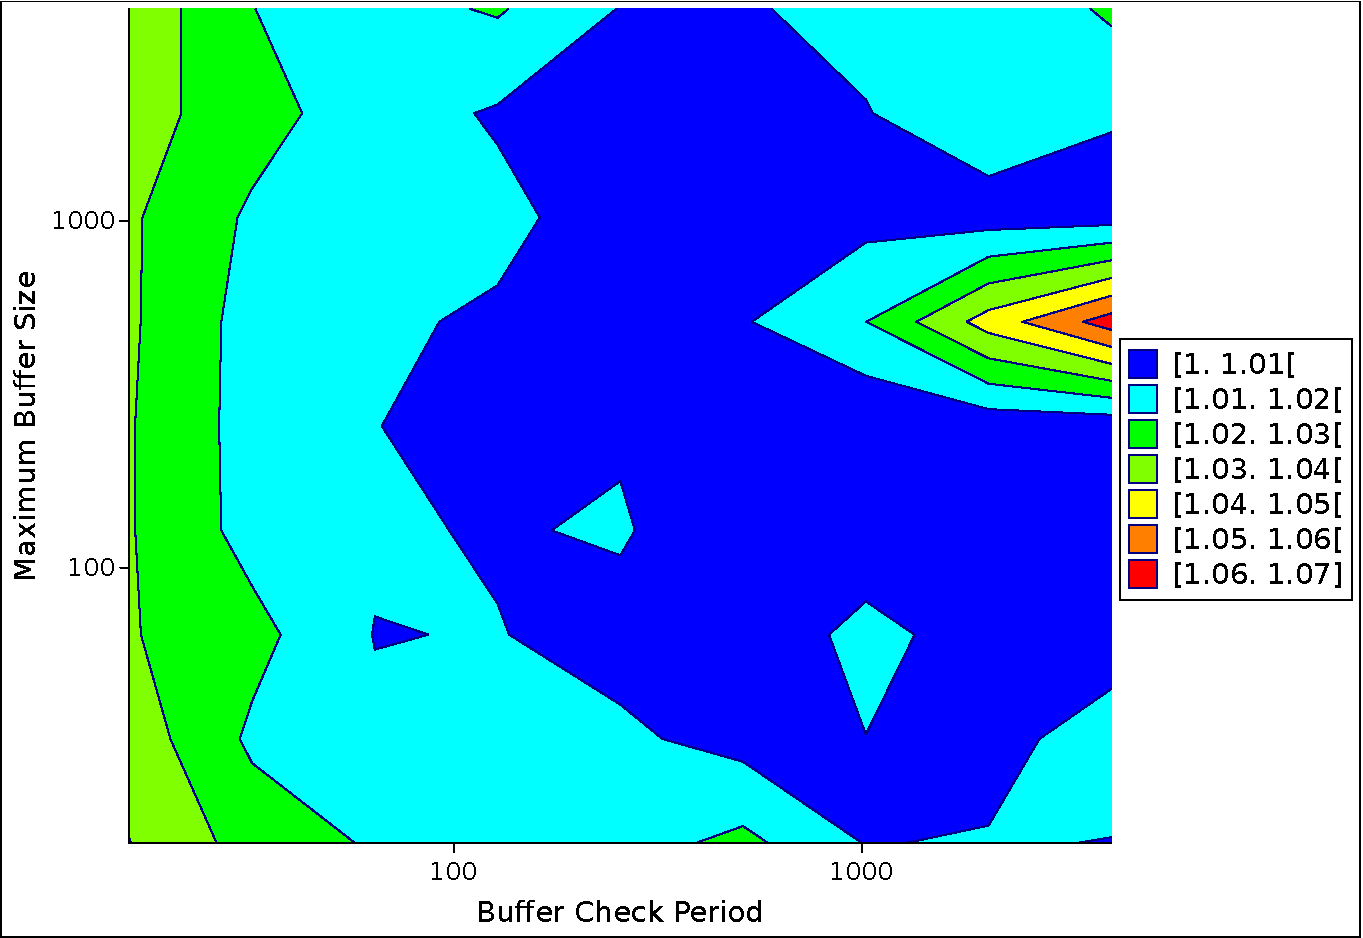
\includegraphics[width=6in]{chapters/parallel_mc/titan_comm_parameters.pdf}
  \end{center}
  \caption{\textbf{Neumann Ulam parallel algorithm history buffer
      check period vs. history buffer size sensitivity.} \textit{The
      color scale represents the ratio of the runtime of a particular
      parameter variation with the runtime from the faster parameter
      variation. A value of 1.02 on the color scale corresponds to a
      runtime 2\% longer than the faster time. All runtimes were
      within 6.5\% of the fastest observed case.}}
  \label{fig:titan_comm_parameters}
\end{figure}

Compared to the reference work, there was also not a significant
change in the runtime over the values of parameters tested with all
runtimes reported within 6.5\% of the fastest case observed. For this
work, a history buffer size of 4096 and a buffer check period of 128
performed best for the initial calculations. However, most values in
the range tested will give good performance. Brunner and Brantley
found that a value of 1024 was best for both parameters. For the
results observed here, these parameters were only 0.7\% slower than
the fastest case. It may be best practice to fix these parameters
internally at 1024 as both this work and the reference found these to
perform well several years apart on both different parallel machines
and for different transport sequences. Therefore, for the scaling
studies presented in the following sections, values of 1024 for both
the history buffer size and message check frequency will be used.

\clearpage

\subsection{Pure Domain Decomposition Scaling}
\label{subsec:pure_domain_decomp}

For the first set of scaling studies, we consider the parallel MCSA
algorithm where MSOD has not been used in the parallel Neumann-Ulam
algorithm. We refer to this case as pure domain decomposition where no
overlap or replication has been leveraged. Such a test will isolate
specifically the performance of Brunner and Brantley's algorithm as
applied to the Neumann-Ulam algorithm. For the strong scaling study,
the global diffusion problem size was fixed at \sn{1.6}{7} DOFs for
all solvers and the 16 core run used as the base case. MCSA was used
again with one stochastic history used per DOF in the Neumann-Ulam
solve to compute the correction for the acceleration with the
remainder of the problems and solver parameters the same as those for
the verification calculation given in
Table~\ref{tab:parallel_verification_parameters} and
Table~\ref{tab:parallel_mcsa_parameters}. As with all of the scaling
studies, 3 calculations for all data points were performed with the
average wall time reported and used for the efficiency
calculations. Figure~\ref{fig:titan_pure_strong_time} gives the wall
time per iteration for these calculations while
Figure~\ref{fig:titan_pure_strong} gives the results of the this study
with the given absolute efficiencies computed using
Eq~(\ref{eq:strong_scaling_absolute}). We report wall time per
iteration due to the fact that MCSA converged on the solution in 22
iterations while the Krylov solvers converged in 19 iterations.

\begin{figure}[t!]
  \begin{center}
    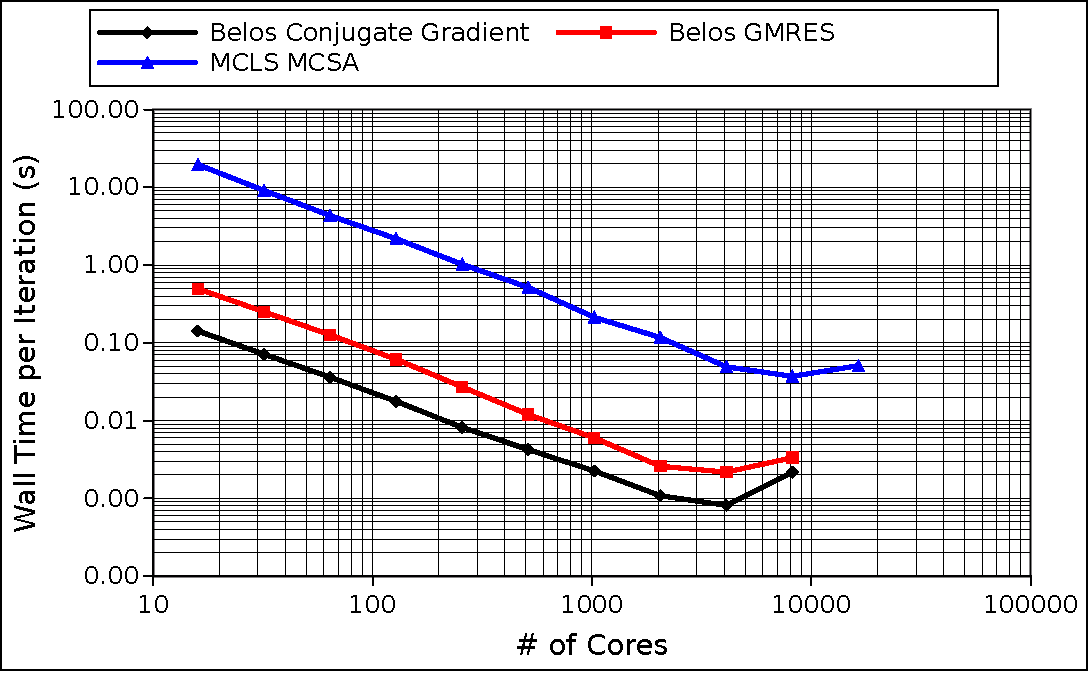
\includegraphics[width=6in]{chapters/parallel_mc/titan_pure_strong_time.pdf}
  \end{center}
  \caption{\textbf{Pure domain decomposition strong scaling wall time
      per iteration.} \textit{Wall time is reported per iteration
      because the methods converged in different numbers of
      iterations. MCLS is over an order of magnitude slower
      arithmetically than the Krylov solvers. GMRES executes more
      operations than conjugate gradient and is therefore slower as
      well.}}
  \label{fig:titan_pure_strong_time}
\end{figure}

\begin{figure}[t!]
  \begin{center}
    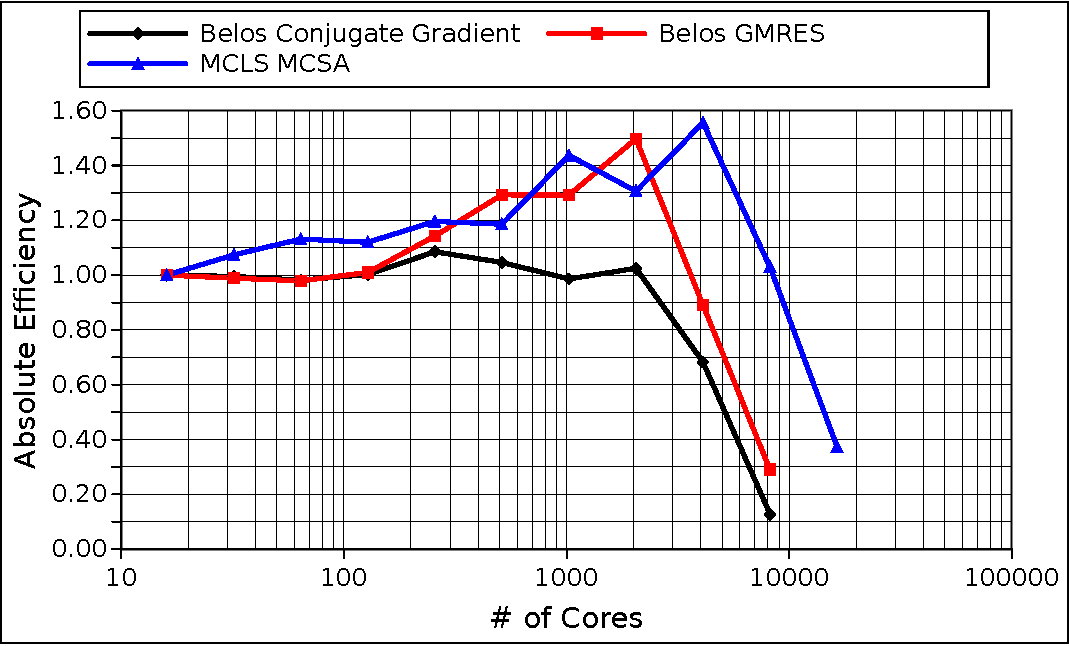
\includegraphics[width=6in]{chapters/parallel_mc/titan_pure_strong.pdf}
  \end{center}
  \caption{\textbf{Pure domain decomposition strong scaling absolute
      efficiency.}  \textit{Super-linear speed-up is from memory
      thrashing in the base case. MCLS is over an order of magnitude
      slower arithmetically, causing the higher efficiency. GMRES
      executes more operations than conjugate gradient, also creating
      a higher efficiency.}}
  \label{fig:titan_pure_strong}
\end{figure}

There are several key features of
Figure~\ref{fig:titan_pure_strong_time} and
Figure~\ref{fig:titan_pure_strong} worth noting. First, up to around
5,000 cores, all methods experience a super-linear improvement in
parallel efficiencies. For all methods, this increase is not a
function of the algorithmic efficiency as those computed using
Eq~(\ref{eq:algorithmic_efficiency}) remained at unity, meaning that
all computations converged in the same number of iterations relative
to the base case\footnote{When the algorithmic efficiency remains at
  unity for all calculations, the implementation efficiency is
  equivalent to the absolute efficiency and therefore is not presented
  here.}. Instead, what is happening here and was observed by Brunner
and Brantley in their work is that the large problem used to scale to
O(10,000) cores was large enough that memory thrashing was occurring
in the 16 core base case. As the number of cores in the strong scaling
study was increased and the local problem size decreased, more of the
local problem fit into the cache of the system, thus causing improved
serial performance and therefore enhanced runtimes. In this region of
super-linear efficiencies, we also observe larger efficiencies for
GMRES as compared to conjugate gradient. This occurs due to the fact
that conjugate gradient has a static set of operations performed at
every iteration while GMRES operates on a continually growing
subspace. In addition, the orthogonalization operations required to
generate that subspace consume much more time than the basic conjugate
gradient operations, causing a larger serial runtime and subsequently
higher efficiencies. For the same reasons, we also observe higher
efficiencies for the MCSA implementation due to the serial performance
of the implementation.

Beyond around 5,000 cores, the global problem size selected for this
strong scaling study causes the local problem size to shrink enough
that parallel communication costs begin to overtake arithmetic costs
on process. This takeover causes this effective strong scaling wall
that is observed in all methods. Using any more cores to solve this
particular global problem is not an efficient use of those parallel
resources. Furthermore, the fact that we see a very similar trends in
efficiencies for all methods means that they are bound by the same
parallel performance limitations in a strong scaling environment. This
is important as we can expect the same qualitative scaling performance
from MCSA if arithmetic optimization has been performed to improve the
serial performance of the implementation. In addition, these results
are valuable in that they show MCSA, when properly parallelized, has
the ability to be competitive on leadership-class computing platforms
with conventional subspace methods with good strong scaling observed
in the pure domain decomposition case to O(10,000) cores.

Next, we consider the weak scaling performance of the algorithm. In
this case, we fix the local problem size at \sn{4}{4} DOFs and
increase the number of processors used in the
simulation. Figure~\ref{fig:titan_pure_weak_time} gives the wall
time per iteration and Figure~\ref{fig:titan_weak_absolute} gives the
weak scaling absolute efficiencies for this problem as computed by
Eq~(\ref{eq:weak_scaling_absolute}). In general, the relative trends
when comparing MCSA to the Krylov methods are the same with MCSA and
GMRES scaling better than the conjugate gradient method due to the
increased amount of arithmetic work on-process. In addition, it is
important to note that the weak scaling of MCSA when properly
parallelized remains competitive with the Krylov methods keeping in
mind the artificial inflation of efficiencies.

\begin{figure}[t!]
  \begin{center}
    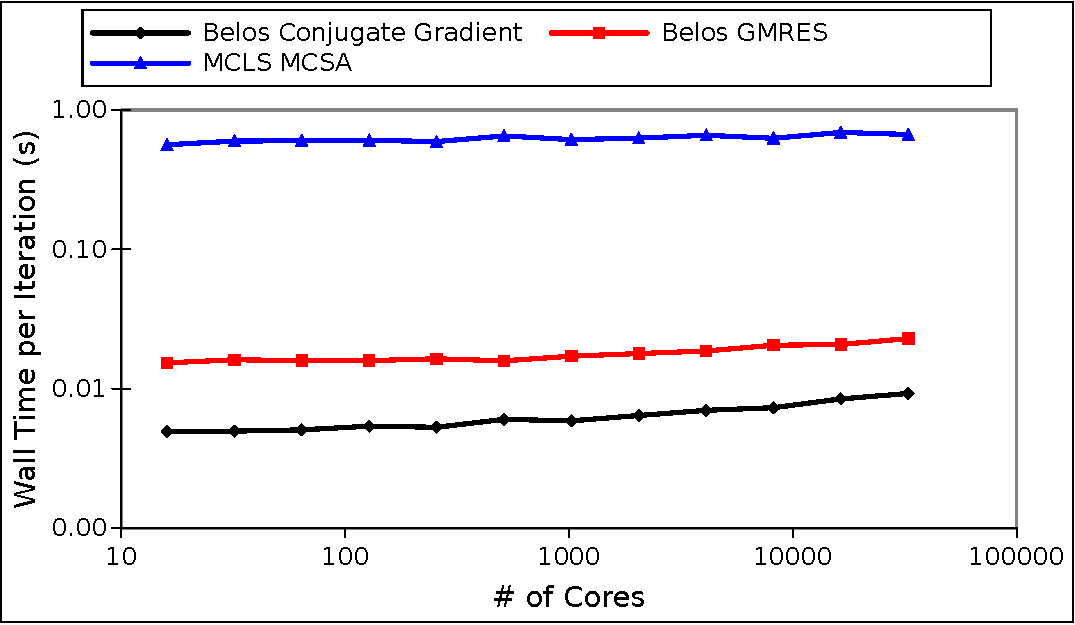
\includegraphics[width=6in]{chapters/parallel_mc/titan_pure_weak_time.pdf}
  \end{center}
  \caption{\textbf{Pure domain decomposition weak scaling wall time
      per iteration.} \textit{Wall time is reported per iteration
      because the methods converged in different numbers of
      iterations. MCLS is over an order of magnitude slower
      arithmetically than the Krylov solvers. GMRES executes more
      operations than conjugate gradient and is therefore slower as
      well.}}
  \label{fig:titan_pure_weak_time}
\end{figure}

\begin{figure}[t!]
  \begin{center}
    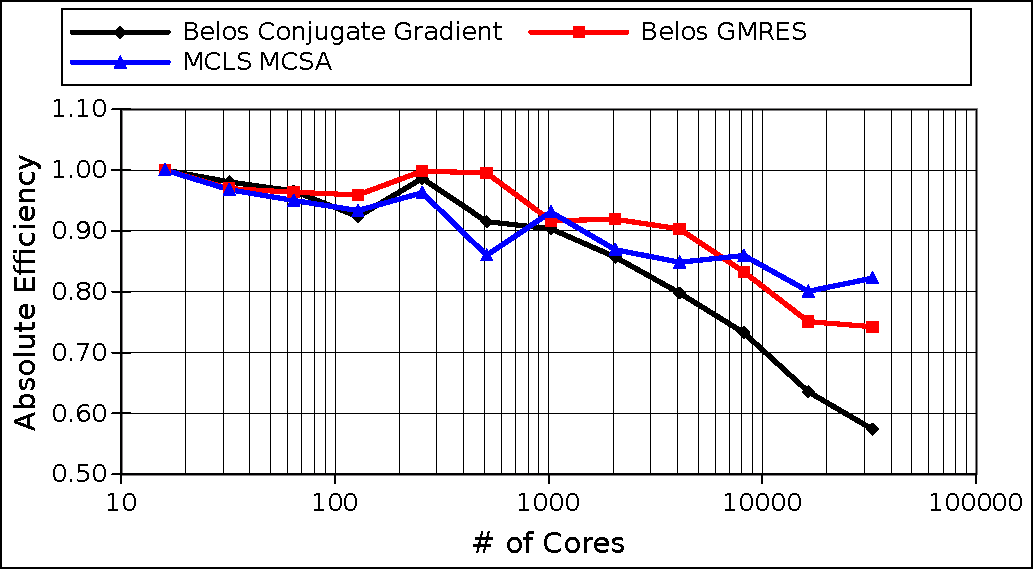
\includegraphics[width=6in]{chapters/parallel_mc/titan_weak_absolute.pdf}
  \end{center}
  \caption{\textbf{Pure domain decomposition weak scaling absolute
      efficiency.} \textit{MCLS is an over order of magnitude slower
      arithmetically, causing the higher efficiency. GMRES executes
      more operations than conjugate gradient, also creating a higher
      efficiency.}}
  \label{fig:titan_weak_absolute}
\end{figure}

As an additional means of comparison between MCSA and the Krylov
methods, we compute the algorithmic efficiencies of the calculations
using Eq~(\ref{eq:algorithmic_efficiency}). As shown in
Figure~\ref{fig:titan_weak_algorithmic}, the algorithm efficiency of
the Krylov algorithm improves as a function of the number of cores in
the problem due to the fact that the number of iterations required to
converge decreased from 20 in the base case to 19 and then to 18 for
the final set of weak scaling computations. When this reduction in
iterations is used to account for the observed runtimes and computed
absolute efficiencies for weak scaling we end up with the
implementation efficiencies computed using
Eq~(\ref{eq:implementation_efficiency}) given in
Figure~\ref{fig:titan_weak_implementation}. Because MCSA maintains the
same iterative performance as a function of global problem size in the
weak scaling study, the implementation efficiencies compare more
favorably to the Krylov methods. Using the implementation efficiency,
we are effectively measuring the parallel performance of a single
iteration for each method by looking at these implementation
efficiencies. As the global problem size increases, MCSA is less prone
to a drop in parallel efficiency. If optimization has been performed
and runtimes potentially approach those of the Krylov methods, this
comparison may not be as favorable. Overall, weak scaling performance
of the parallel MCSA algorithm is excellent for the pure domain
decomposition case with absolute parallel efficiencies of over 80\%
observed at over 32,000 cores.

\begin{figure}[t!]
  \begin{center}
    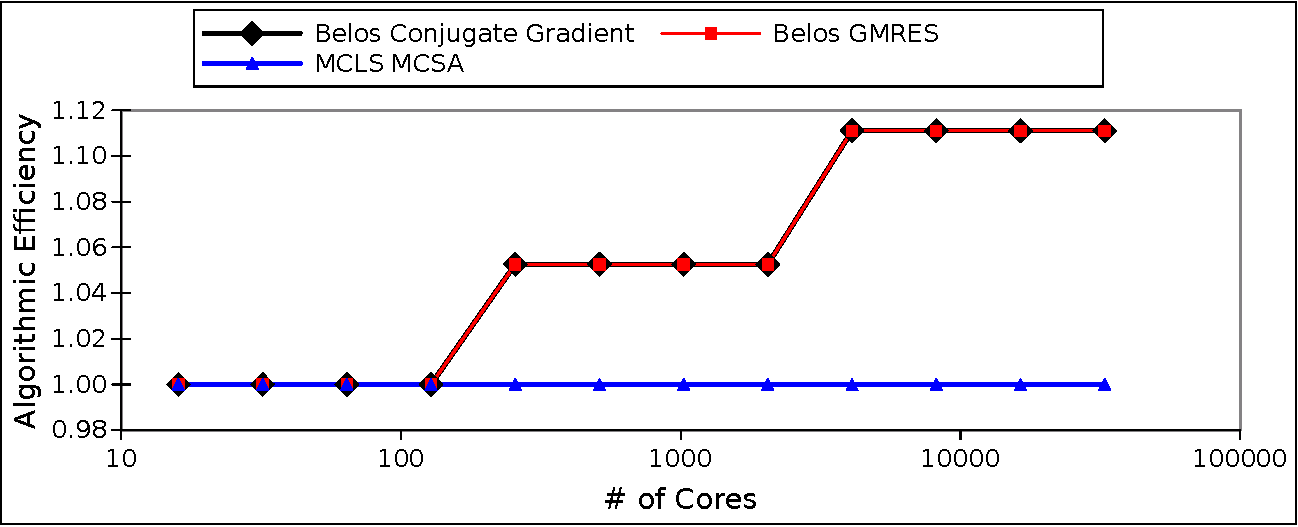
\includegraphics[width=6in]{chapters/parallel_mc/titan_weak_alg_eff.pdf}
  \end{center}
  \caption{\textbf{Pure domain decomposition weak scaling algorithmic
      efficiency.} \textit{As the global problem size was increased in
      the weak scaling study, both conjugate gradient and GMRES
      converged in fewer iterations, causing the rise in algorithmic
      efficiency.}}
  \label{fig:titan_weak_algorithmic}
\end{figure}

\begin{figure}[t!]
  \begin{center}
    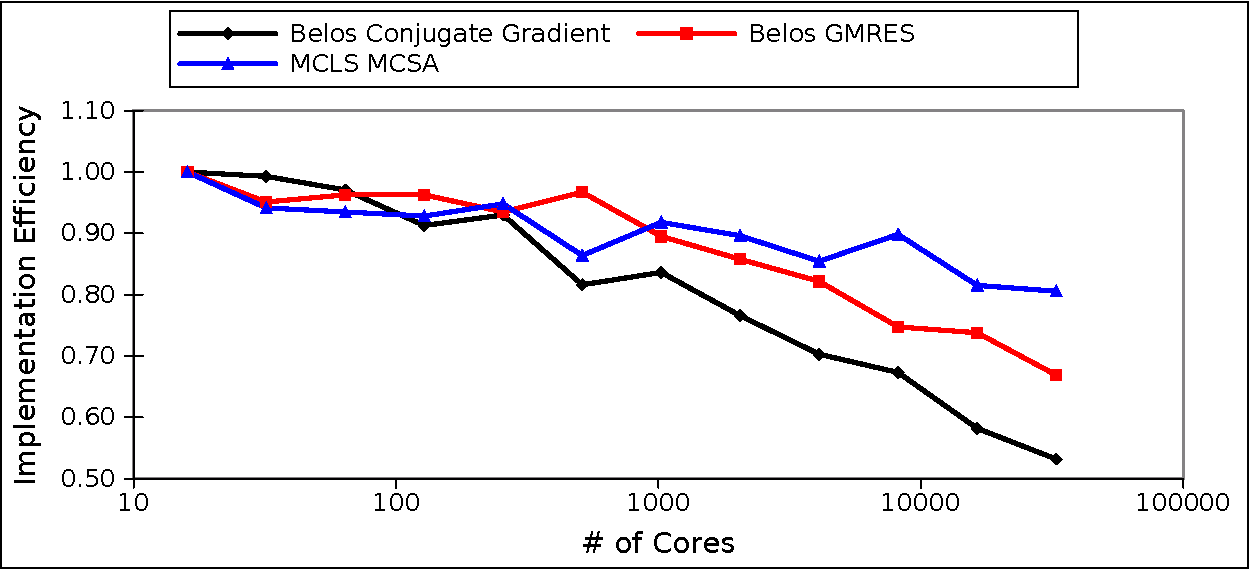
\includegraphics[width=6in]{chapters/parallel_mc/titan_weak_implementation.pdf}
  \end{center}
  \caption{\textbf{Pure domain decomposition weak scaling
      implementation efficiency.} \textit{Considering the scalability
      of a single iteration of the implementation, the inflated
      efficiencies of the MCLS MCSA implementation become more
      obvious. Implementation optimization will likely reduce the MCSA
      values to a level more comparable to the Belos values.}}
  \label{fig:titan_weak_implementation}
\end{figure}

In addition to comparing MCSA scaling to conventional methods, we also
motivate avoiding any type of master/slave algorithms at these high
levels of concurrency by comparing the binary communication tree
implementation used in the previous results with a parallel MCSA
implementation that uses the master/slave scheme to determine the end
of a history transport stage as shown in
Figure~\ref{fig:master_comm_tree}
instead. Figure~\ref{fig:titan_strong_bvsm} provides this comparison
using the strong scaling study while Figure~\ref{fig:titan_weak_bvsm}
gives the results of the comparison for the weak scaling study. In
both cases, the deficiencies caused by using the master/slave scheme
for transport completion are obvious. At around 1,000 cores, both the
strong and weak scaling performance seriously degrades while the
binary tree pattern maintains excellent performance. At this number of
cores, any extra work given to the master process, even if it amounts
to summing a handful of integers and checking for a few extra messages
as in this algorithm, grows enough to create serious load imbalance
and reduce performance.

\begin{figure}[t!]
  \begin{center}
    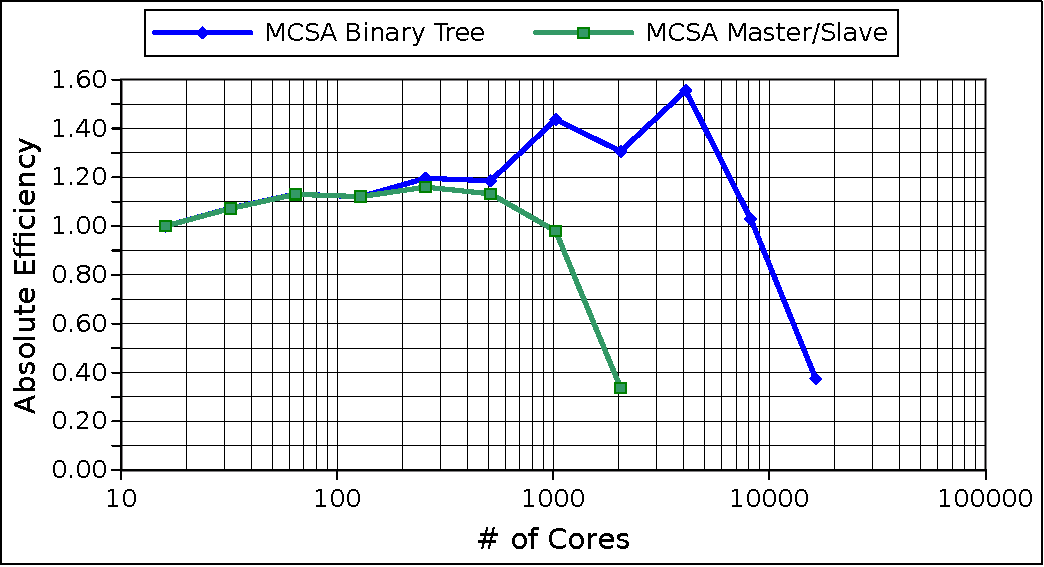
\includegraphics[width=6in]{chapters/parallel_mc/titan_strong_bvsm.pdf}
  \end{center}
  \caption{\textbf{Binary tree vs. master/slave communication scheme
      strong scaling absolute efficiency.} \textit{The master/slave
      scheme will not scale beyond $O(1,000)$ cores due to load
      imbalance.}}
  \label{fig:titan_strong_bvsm}
\end{figure}

\begin{figure}[t!]
  \begin{center}
    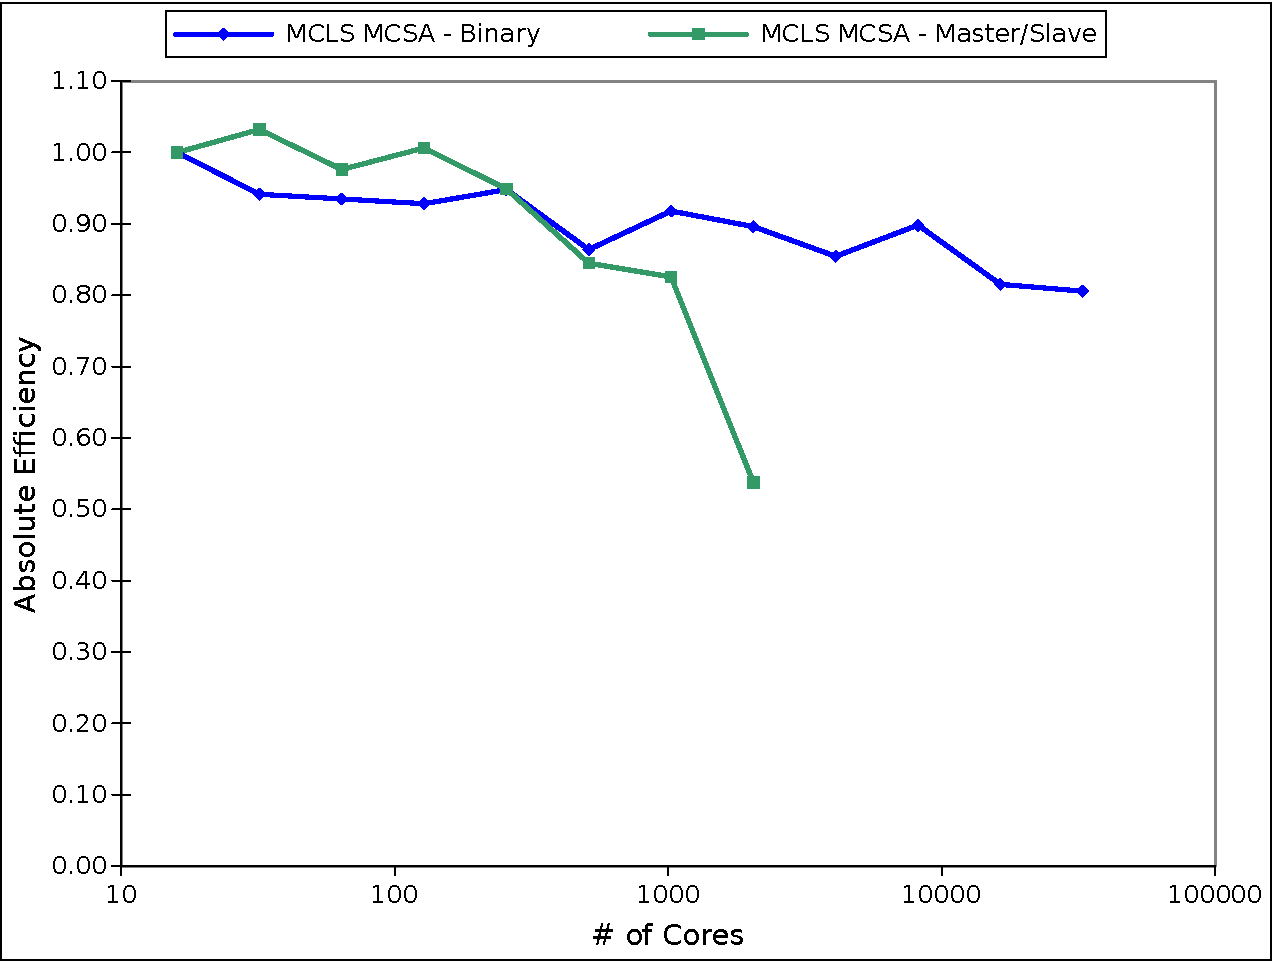
\includegraphics[width=6in]{chapters/parallel_mc/titan_weak_bvsm.pdf}
  \end{center}
  \caption{\textbf{Binary tree vs. master/slave communication scheme
      weak scaling absolute efficiency.}  \textit{The master/slave
      scheme will not scale beyond $O(1,000)$ cores due to load
      imbalance.}}
  \label{fig:titan_weak_bvsm}
\end{figure}

\clearpage

\subsection{Overlapping Domain Decomposition}
\label{subsec:overlapping_domain_decomp}

In the next set of scaling studies, we will explore how adding overlap
to the subdomains in the problem affects runtimes and parallel
performance as compared to the case with pure domain decomposition. To
do this, we utilize the set of analytic relations developed in
\S~\ref{sec:analytic_framework} to design these numerical
experiments. For the neutron diffusion problem used in these scaling
studies, the linear operator had a spectral radius of 0.787 and a
weight cutoff of \sn{1}{-2} was used with the Neumann-Ulam
solver. Using Eq~(\ref{eq:analytic_k}) gives an expected random walk
length of 19.22 transitions for any given history in the
problem. Using the mean-chord approximation given by
Eq~(\ref{eq:mean_chord_domain_leakage}), we then expect approximately
5.3\% of the histories born in a particular domain to leak out after
the first transport stage. By adding overlap, we aim to reduce this
fraction of communicated histories and therefore boost the parallel
performance of the algorithm. 

To determine the amount of overlap to test for the scaling studies, we
use a variation of Eq~(\ref{eq:step_k_length}) to determine how many
discrete states a history will move on average from its birth site. We
modify Eq~(\ref{eq:step_k_length}) to only account for discrete
movements:
\begin{equation}
  \sqrt{\bar{n^2_k}} = n_s \sqrt{k}\:,
  \label{eq:discrete_distance}
\end{equation}
where $\sqrt{\bar{n^2_k}}$ is now the root-mean-squared number of
discrete states a history will move from its birth site. For our
diffusion problem used in these scaling studies, we compute a value of
2.63 states per history for any of the dimensions of the system. This
means that we can expect to end up on average 2.63 states in both the
$i$ and $j$ dimensions away from the starting state. Therefore, we
will use the overlap generation algorithm outlined in
\S~\ref{subsec:msod_generation} such that we parametrically grow the
local domain using 1, 2, 3, and 5 levels to measure how scalability is
affected when this root-mean-squared number of states is
considered. For example, using 3 levels of overlap should keep over
50\% of the histories that would be communicated in the pure domain
decomposition case on-process as this is greater than the
root-mean-squared number of states we would expect a history to
travel.

For the performance metrics, we may use the same weak and strong
scaling efficiency metrics that we used for the pure domain
decomposition case. As we are comparing to the case without overlap
and are looking to boost performance relative to the case without
overlap, for both weak and strong scaling calculations we will use the
16-core case without overlap as the reference computation for all
efficiency measures reported. 

The absolute efficiency results from the strong scaling exercise are
given in Figure~\ref{fig:titan_strong_overlap}. Aside from the
boosting of efficiencies at 2,048 cores, little evidence of strong
scaling improvement is evident for all levels of overlap tested. To
further explore any potential benefits of adding overlap into the
system, Figure~\ref{fig:titan_strong_overlap_diff} gives the
difference in the efficiencies between all overlap cases and the
reference case without overlap at each core count. At smaller numbers
of cores, there is no observed benefit to using overlap to improve
strong scaling. The improvements noted at 2,048 cores are also present
here and account for the best efficiency improvements for all core
counts tested. at 16,384 cores, using 2 levels of overlap did give a
6.4\% boost in efficiency while at 1,024 cores this same amount of
overlap actually reduced the efficiency. Beyond 2 levels of overlap,
efficiency levels begin to fall with 5 levels of overlap performing
the worst for all cases. From this, we don't expect adding any more
overlap will improve the scalability of the algorithm and the best
strong scaling performance was observed when the number of overlap
levels is approximately equal to the root-mean-squared number of
states we expect a history to move from its starting point as computed
by Eq~(\ref{eq:discrete_distance}). We will defer an explanation of
the drop in efficiencies for levels of overlap beyond this value until
we have analyzed the weak scaling data.

\begin{figure}[t!]
  \begin{center}
    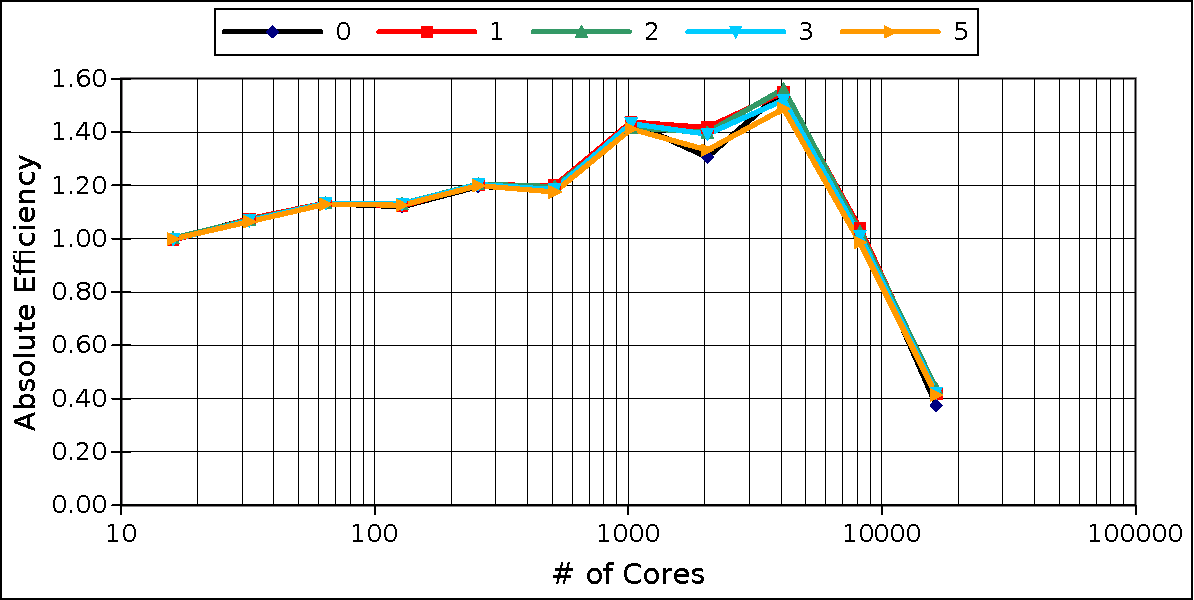
\includegraphics[width=6in]{chapters/parallel_mc/titan_strong_overlap.pdf}
  \end{center}
  \caption{\textbf{Strong scaling absolute efficiency with varying
      levels of overlap.} \textit{Values of 0, 1, 2, 3, and 5 levels
      of overlap were used as the problem had a root-mean-squared
      number of states of 2.63 for each history.}}
  \label{fig:titan_strong_overlap}
\end{figure}

\begin{figure}[t!]
  \begin{center}
    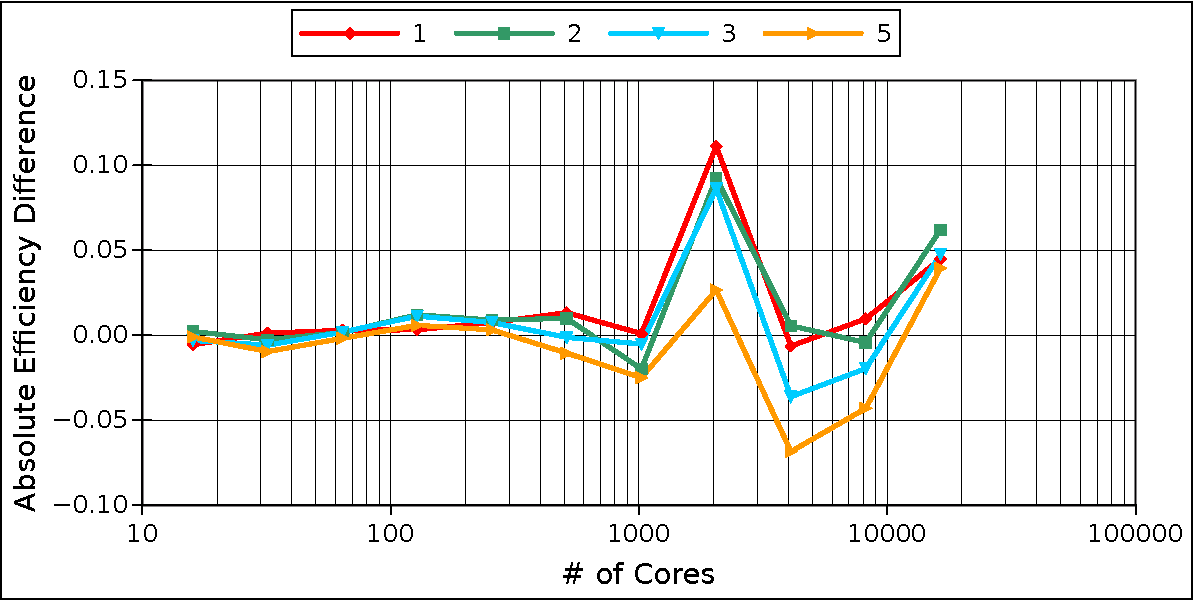
\includegraphics[width=6in]{chapters/parallel_mc/titan_strong_overlap_diff.pdf}
  \end{center}
  \caption{\textbf{Strong scaling absolute efficiency difference with
      respect to the 0 overlap base case.} \textit{Values of 1, 2, 3,
      and 5 levels of overlap are compared here with the absolute
      difference of the absolute efficiencies presented.}}
  \label{fig:titan_strong_overlap_diff}
\end{figure}

For weak scaling, the same study as in the pure domain decomposition
case was performed again with 1, 2, 3, and 5 levels of overlap. The
absolute parallel efficiencies from these calculations are given in
Figure~\ref{fig:titan_weak_overlap} and the differences in
efficiencies from the calculations without overlap. The results here
are much the same in that there is not a dramatic improvement in
scalability relative to the case without overlap. Opposite the strong
scaling calculation, overlap enhances weak scaling efficiencies at
lower core counts and degrades the efficiencies at higher core
counts. In addition, 1 level of overlap provided the best enhancement
of scalability when overlap was beneficial. 

\begin{figure}[t!]
  \begin{center}
    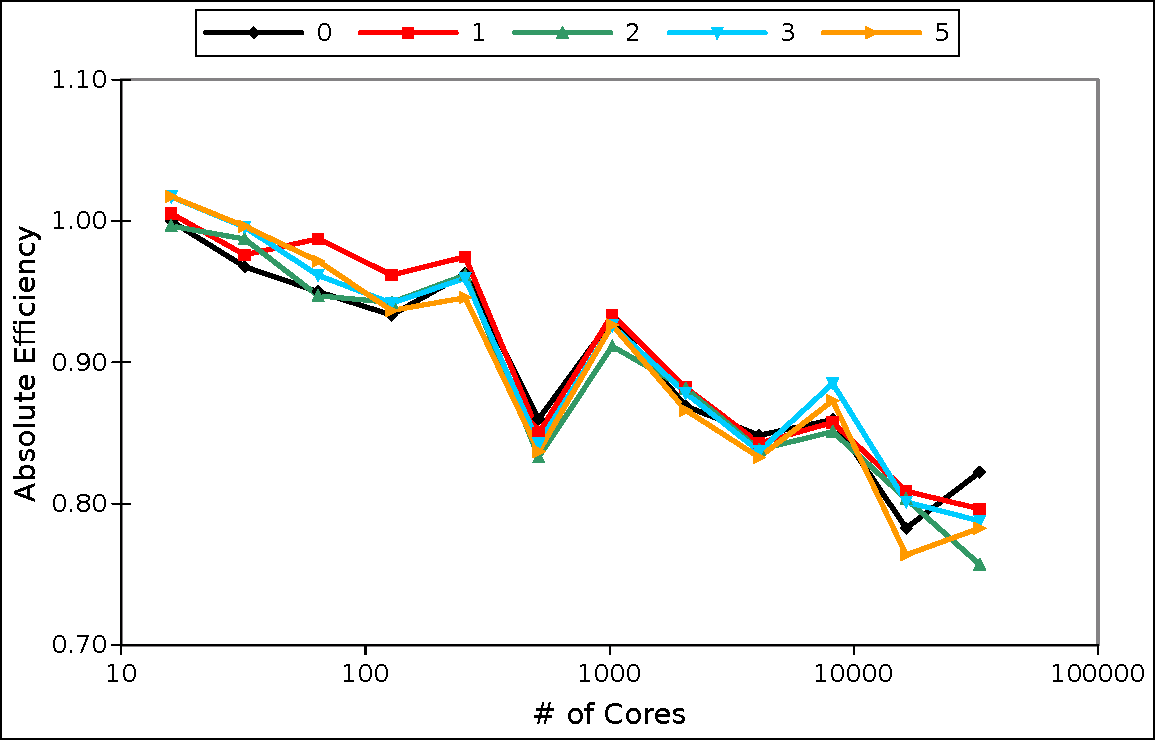
\includegraphics[width=6in]{chapters/parallel_mc/titan_weak_overlap.pdf}
  \end{center}
  \caption{\textbf{Weak scaling absolute efficiency with varying
      levels of overlap.} \textit{Values of 0, 1, 2, 3, and 5 levels
      of overlap were used as the problem had a root-mean-squared
      number of states of 2.63 for each history.}}
  \label{fig:titan_weak_overlap}
\end{figure}

\begin{figure}[t!]
  \begin{center}
    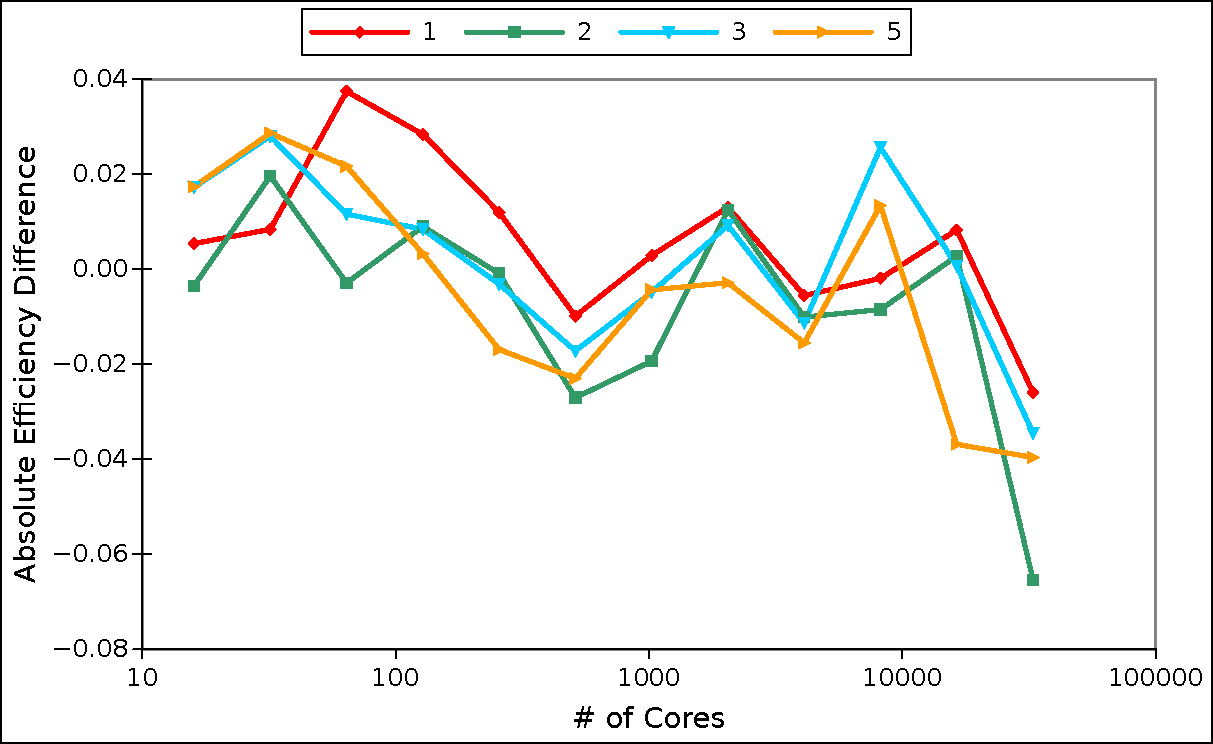
\includegraphics[width=6in]{chapters/parallel_mc/titan_weak_overlap_diff.pdf}
  \end{center}
  \caption{\textbf{Weak scaling absolute efficiency difference with
      respect to the 0 overlap base case.} \textit{Values of 1, 2, 3,
      and 5 levels of overlap are compared here with the absolute
      difference of the absolute efficiencies presented.}}
  \label{fig:titan_weak_overlap_diff}
\end{figure}

For both the strong and weak scaling studies, the parallel performance
of the algorithm was either marginally improved or not improved at
all. We would always expect an improvement in performance for using
overlap to prevent the transport of histories from domain to domain
during execution of the Neumann-Ulam algorithm. The reduction in
transport means a reduction in parallel communication and therefore
should never degrade the performance of the algorithm. It is true that
doing so in fact enhances Monte Carlo performance. However, the
Neumann-Ulam algorithm is not representative of the entire MCSA
algorithm. When overlap is used, an overlapping tally vector is
constructed in parallel such that multiple cores may own multiple
states in the system. When this occurs, the tally data associated with
these shared states must be communicated after the Neumann-Ulam solve
as outlined in \S~\ref{subsec:msod_algorithm}. This reduction
operation then builds the full MCSA correction vector in the
decomposition of the solution vector. 

Therefore, by building overlap we are in fact reducing parallel
communication during the Neumann-Ulam solve but we are simply
deferring that communication until after Monte Carlo transport when
the overlapping tally vector must be reduced. When overlap becomes
large enough (i.e. larger than the root-mean-squared number of
discrete states a history will travel), then the savings in
communication during the Neumann-Ulam solve start to become smaller
than the communication created in the overlapping tally vector
reduction. We see this in both the strong and weak scaling cases at
larger levels of overlap. For the strong scaling case, we see better
performance improvement at higher core counts because the total number
of overlapping states on each core is smaller from the local problem
size shrinking. For weak scaling, we see better performance
improvement at lower numbers of cores because although the local
overlap size is fixed, the global amount of overlap is growing with
core count and therefore reducing the performance of the tally
reduction operation. 

Based on this data, a few levels of overlap within the expected
distance of travel for a history may offer some marginal improvement
in scalability, however, it is not as effective as one might think
given its improvement to reactor physics calculations as observed in
the literature. This is largely due to the density of states in the
system that creates the described performance bottlenecks in the
overlapping tally vector reduction operation. In a Monte Carlo
particle simulation, these overlapping tally reduction operations are
not expected to be performed at the speed they are required in
MCSA. For example, in a criticality calculation with overlapping
domains, we would expect to perform as many parallel tally vector
reduction in a particle transport simulation as there are particle
stages required for convergence of the eigenvalue. However, these
particle stages will likely be much more costly in terms of wall time
relative to a Neumann-Ulam solve in an MCSA iteration due to the more
extensive particle physics and logic structure that must be
evaluated. Therefore, we can expect this overlapping tally reduction
to be less significant to scalability in those operations. We do not
have as complicated a logic structure in a history random walk for the
Neumann-Ulam method and therefore overlap can inhibit scalability if
too large.

\clearpage

\subsection{Multiple Set Domain Decomposition}
\label{subsec:ms_decomposition}

We next look to apply replication to the problem in the form of
multiple sets. As the previous analysis showed overlap to be of little
assistance in improving scalability, we only apply multiple sets to
the problem with pure domain decomposition within the sets for these
scaling studies. Before performing parallel scaling studies using
multiple sets, several aspects of the replicated parallel problem must
be considered in order to effectively craft the studies and interpret
their results. First is the question of how many stochastic histories
to use to generate the correction vector in the MCSA iteration. For
this work we consider two choices; the split case and the fully
replicated case. As an example of these cases, consider a single set
problem where 20,000 histories are used in the Monte Carlo solve. If
we choose the split case, then solving the same problem with 2 sets
would give 10,000 histories in each set and 4 sets would give 5,000
histories in each set. Splitting the histories in this way provides
the same global number of histories used to compute the correction in
the single set problem. We expect to reduce the time to solution by
doing this as each individual set solve will occur faster in an almost
linear fashion with the reduced number of histories. For the
replicated history case, each additional set in the problem will use
just as many histories as the single set case. Using 2 sets with fully
replicated histories for our example problem then has each set
computing 20,000 histories with 40,000 global histories in the
computation. For the 4 set case, the number of global histories is
increased to 80,000. We also expect this type of replication to reduce
the time to solution as the extra global histories should reduce the
stochastic uncertainty in the correction vector and reduce the overall
number of MCSA iterations required to converge.

\subsubsection{Strong Scaling with Multiple Sets}
\label{subsubsec:ms_strong}

For the strong scaling study, we apply the additional sets as
follows. Using the same problems as the pure domain decomposition
scaling study, the multiple sets are used to replicate those problems
and boost the core count. For example, for the 4 set case, the data
point at 64 cores has the same $N/P$ ratio in one set as the single
set problem with 16 cores. This is due to the fact that $N$ is fixed
for the strong scaling study and 4 replications gives a set size of 16
cores. For the 2 set case, the 32 core data point is solving the same
$N/P$ problem in a set as the 16 core base case.

In addition to considering the replicated domain, we must also
consider how to modify the efficiencies we will compute. For the
strong scaling case, recall that the objective is to decrease the time
to solution for a given global problem size $N$ by increasing
$P$. Therefore, we may use Eqs~(\ref{eq:strong_scaling_absolute_ref}),
(\ref{eq:algorithmic_efficiency}), and
(\ref{eq:implementation_efficiency}) to compute the various strong
scaling efficiencies, but we must modify the reference computation in
each of these formulas to reflect our objective. For all efficiency
computations, the 16 core single set computation will be used as the
reference case. By adding more cores to the problem, either by
replicating with multiple sets, or decreasing the local problem size,
any computational resources added to the problem should aim to result
in speedup of this reference case. If this speedup for one technique
of adding cores is less than another, then that technique is deemed a
less efficient use of those computational resources.

For the multiple sets problem, the single set strong scaling study
from the pure domain decomposition base case was repeated for multiple
sets with both splitting of histories across sets and full replication
of histories across sets using both 2 and 4
sets. Figure~\ref{fig:titan_strong_ms_time} gives the actual wall
times for these computations. There are two important features to note
in the wall time data. First, splitting the histories among sets
instead of replicating them is faster due to the fact that cutting the
number of histories in half reduces the time of an iteration by a
factor that is nearly linear while increasing linearly the number of
histories through replication does not decrease the iterations
required to converge by a linear factor. Second, until the strong
scaling wall is hit starting at around 10,000 cores, the single set
case actually performs the fastest with only marginal improvement in
runtimes at higher numbers of cores with more sets. At these larger
numbers of cores, however, the improvements are so modest that one is
better off running the same problem using a single set at lower core
counts to conserve computational resources while maintaining a good
time to solution.

\begin{figure}[t!]
  \begin{center}
    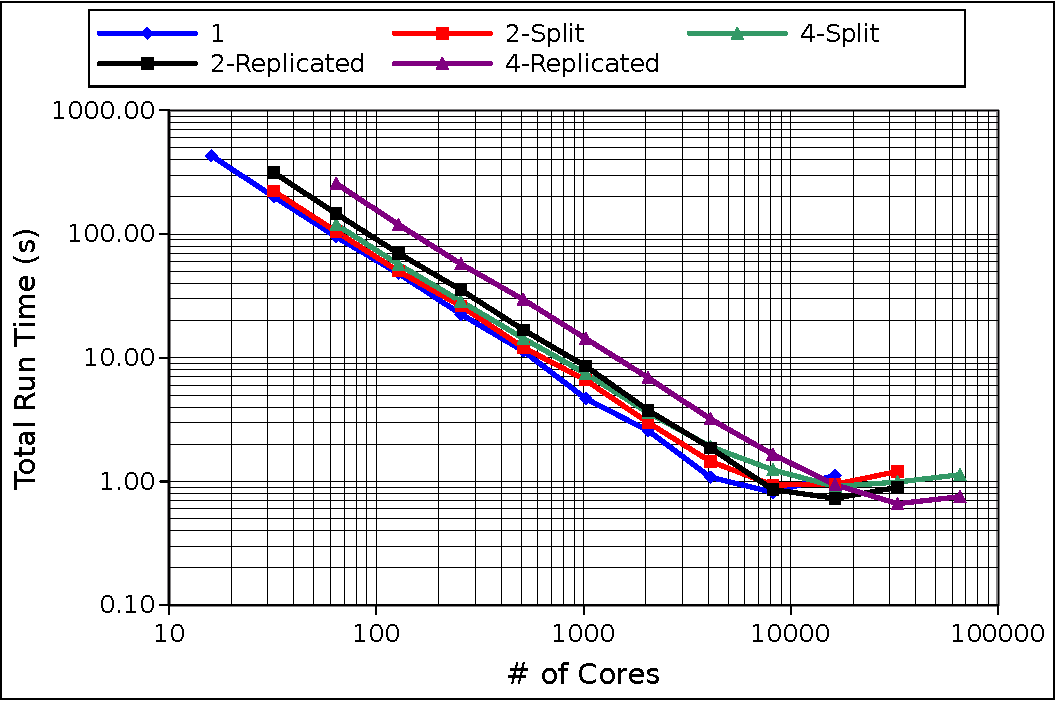
\includegraphics[width=6in]{chapters/parallel_mc/titan_strong_ms_time.pdf}
  \end{center}
  \caption{\textbf{Wall time in seconds to solution for each case for
      the strong scaling study with multiple sets.} \textit{Until the
      strong scaling wall is reached at O(10,000) cores, the single
      set case performs the best. For the multiple set cases, it is
      faster to split histories among sets and maintain iterative
      performance rather than replicate histories to improve iterative
      performance.}}
  \label{fig:titan_strong_ms_time}
\end{figure}

From this timing data we then compute the absolute efficiencies for
strong scaling as given in Figure~\ref{fig:titan_strong_ms_eff} using
the 16-core single set calculation as the reference case. As observed
in the timing data, because the single set case had the fastest run
times up to the strong scaling wall it also has the best observed
efficiencies. For the 2 set case with history splitting, although the
time to perform an iteration was nearly cut in half, the extra
parallel overhead associated with reducing the tally across the blocks
to combine the set results increases run times and reduces
efficiencies. This reduction across blocks is even more obvious for
the 4 set case. For the replicated cases, we do observe a flat region
of parallel efficiencies at larger core counts (up to around 32,000
for the 4 set case with history replication) showing improved scaling
within context of not considering the single set
calculation. Unfortunately, the additional cores do not reduce the
runtime of the global problem as efficiently as expected. Ultimately,
all cases effectively hit the strong scaling wall at the same time at
around O(10,000) cores.

We expect this if we consider the fact that adding sets to the problem
is in itself effectively a form of strong scaling. For any given
problem of fixed size $N$, adding extra sets to the computation
decreases the global ratio of $N/P$ as $P$ will grow with the addition
of sets (although $N/P$ is constant within a set). For the split
history case, the splitting further exacerbates this situation by
further decreasing the amount of histories that will be computed in
the local domain, giving a larger ratio of communication to work in
the Monte Carlo solve. As with with single set results, we also
observe some efficiencies greater than unity for the multiple set
cases also due to improved cache utilization. 

Although not as dramatic as one might originally expect from
introducing replication, there are some modest gains in efficiencies
at high core counts by using multiple sets. Of interest here is where
the multiple set cases perform better than the single set case after
the single set case has hit the strong scaling wall. In
Figure~\ref{fig:titan_strong_ms_eff}, at 16,384 cores the single set
case operates at 38\% efficiency while at the same number of cores,
the 2 set case with history replication operates at 58\%
efficiency. This is reasonable improvement in the use of those
computational resources, gained by replicating the problem. Beyond
16,384 cores, there is not a compelling reason to use more
computational resources for the this problem.

\begin{figure}[t!]
  \begin{center}
    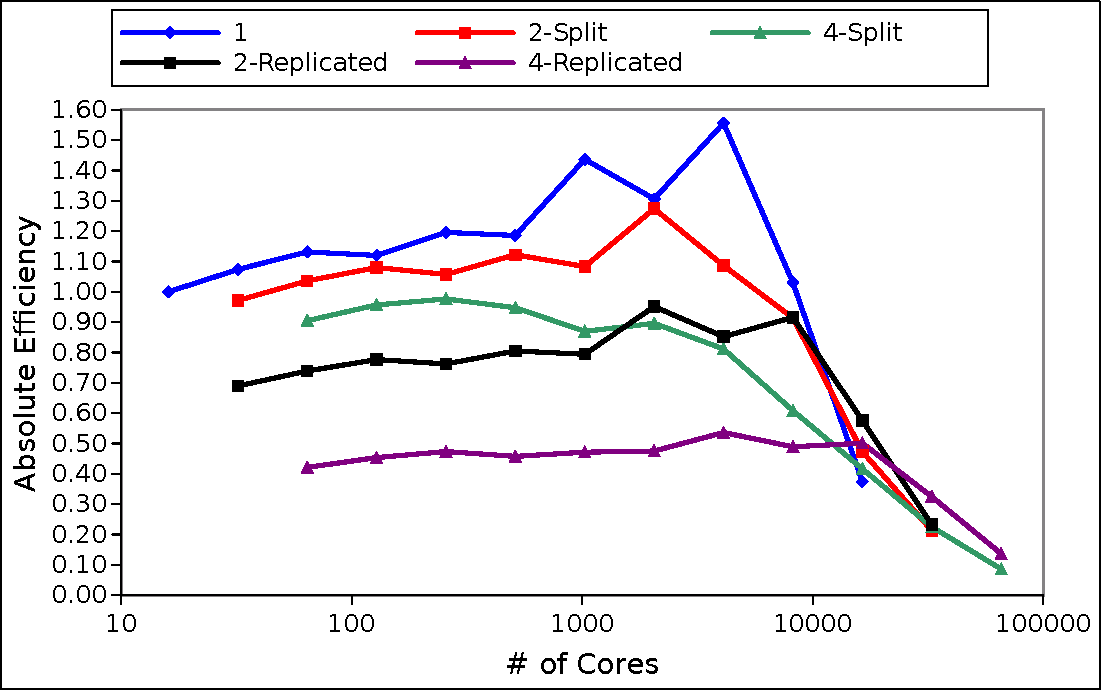
\includegraphics[width=6in]{chapters/parallel_mc/titan_strong_ms_eff.pdf}
  \end{center}
  \caption{\textbf{Multiple set absolute parallel efficiency.}
    \textit{Computed relative to the 16-core 1-set base case. Using a
      single set is the best means by which to improve strong scaling
      up to the strong scaling wall. At higher core counts past where
      the single set case hits the strong scaling wall adding sets can
      provide some improvements in efficiencies.}}
  \label{fig:titan_strong_ms_eff}
\end{figure}

Also of interest here is the effect of splitting histories among sets
versus replicating them on the iterative performance of the
method. Table~\ref{tab:ms_strong_alg_eff} gives the iterations
required to converge and computed algorithmic efficiencies for each of
the cases presented in the strong scaling data. As expected, splitting
histories maintains a fixed global number of histories and therefore
maintained the number of iterations required to converge relative to
the single set base case. When histories were replicated, adding sets
decreased the number of iterations required to converge in a nonlinear
fashion. Therefore, increasing the number of histories per MCSA
iteration improves algorithmic efficiency. Using these algorithmic
efficiencies, the implementation efficiencies for the multiple set
cases were computed and are given in
Figure~\ref{fig:titan_strong_ms_impeff}. From these results, we see
that the replicated history cases are even less efficient than in the
absolute case with respect to the performance of a single
iteration. Not only do we have the additional parallel overhead of
doing the block level reduction, but we also have additional histories
that increase the time to solution for a single iteration.

\begin{table}[h!]
  \begin{center}
    \begin{tabular}{lcc}\hline\hline
      \multicolumn{1}{l}{Case}& 
      \multicolumn{1}{c}{Iterations}&
      \multicolumn{1}{c}{$\eta_{alg}$} \\\hline
      1 & 22 & 1.0 \\
      2-split & 22 & 1.0 \\
      2-replicated & 16 & 1.375 \\
      4-split & 22 & 1.0 \\
      4-replicated & 13 & 1.692 \\
      %%
      \hline\hline
    \end{tabular}
  \end{center}
  \caption{\textbf{Strong scaling algorithmic efficiency using
      multiple sets.} \textit{Replicating histories improves
      algorithmic efficiency by converging in fewer iterations.}}
  \label{tab:ms_strong_alg_eff}
\end{table}

\begin{figure}[t!]
  \begin{center}
    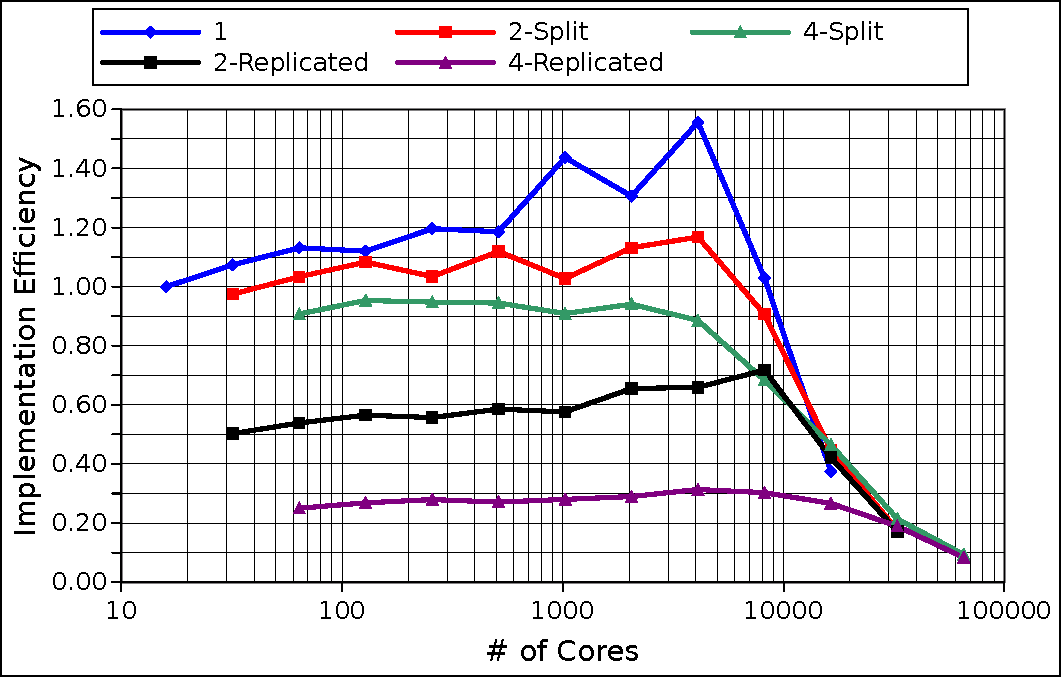
\includegraphics[width=5in]{chapters/parallel_mc/titan_strong_ms_impeff.pdf}
  \end{center}
  \caption{\textbf{Multiple set strong scaling implementation
      efficiency.} \textit{Computed relative to the 16-core 1-set base
      case. Considering iterations required to converge, the
      performance of the split history cases at much better than the
      cases with history replication.}}
  \label{fig:titan_strong_ms_impeff}
\end{figure}

\clearpage

\subsubsection{Weak Scaling with Multiple Sets}
\label{subsubsec:ms_weak}

Next, we continue to a weak scaling study of the multiple sets
problem. In the same way as the strong scaling study, we will modify
the pure domain decomposition study to account for the additional
replication. For each calculation in the single set study, that
problem will be replicated either 2 or 4 times with both split and
replicated histories to assess the effects on scalability and
runtime. Figure~\ref{fig:titan_weak_ms_time} gives the wall times from
the multiple sets weak scaling study. Of primary importance here is
the fact that adding sets to the problem with both split and
replicated histories actually decreases the time to solution. This was
not observed in the strong scaling case until much larger core counts
as the multiple set computations hit the strong scaling wall after the
single set computation.

This result is significant in that it shows a solution technique in
which the linear problem can actually be replicated and enhance time
to solution, something that cannot be achieved with conventional
methods. At larger core counts, however, this reduction in compute
time is not as large as at lower core counts due to the fact that the
tally reduction across blocks requires more resources and those
resources are clearly growing with core count (most obviously in the 4
set case with split histories). In addition, at 131,072 cores for the
largest 4 set computation, load balance is likely becoming an issue
due to the linear system and subsequent parallel matrix and vector
operations only occurring on a subset of the entire processor space of
the problem while the Monte Carlo calculation is occurring on all
processors.

\begin{figure}[t!]
  \begin{center}
    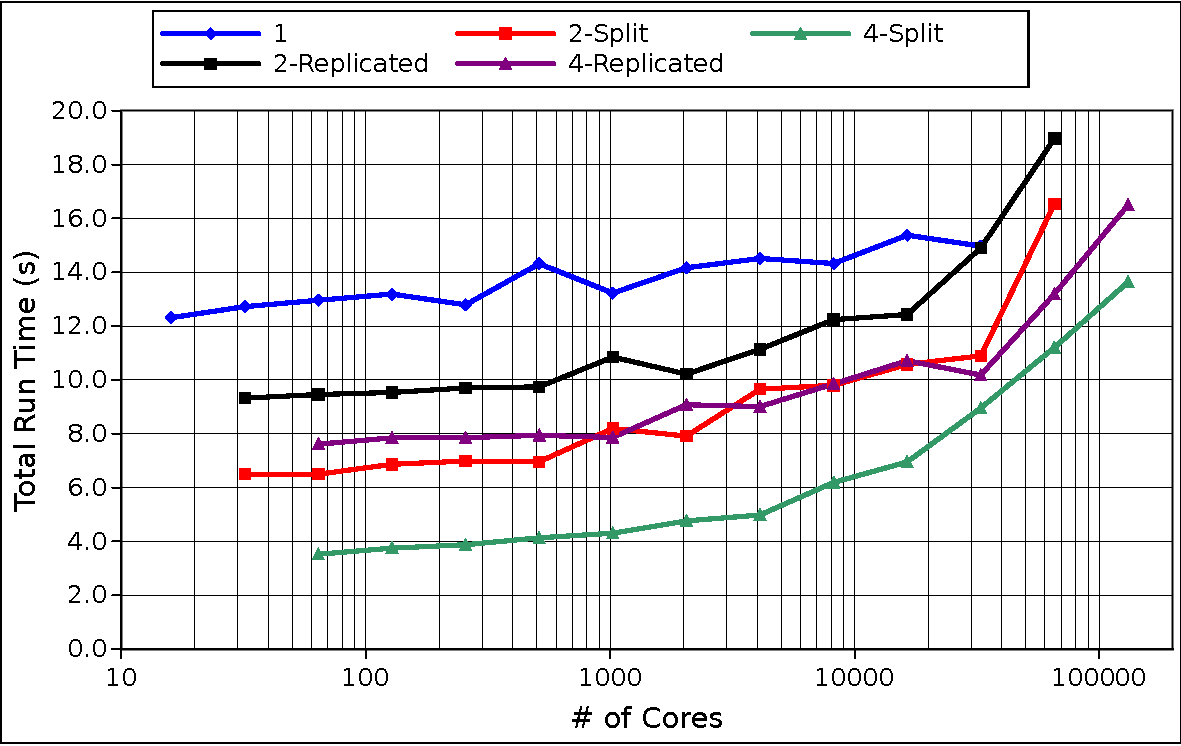
\includegraphics[width=6in]{chapters/parallel_mc/titan_weak_ms_time.pdf}
  \end{center}
  \caption{\textbf{Wall time in seconds to solution for each case for
      the weak scaling study with multiple sets.}}
  \label{fig:titan_weak_ms_time}
\end{figure}

For a multiple set analysis of the weak scaling timing results, we
again have to consider that adding sets to the problem is actually a
form of strong scaling. Consider a single set problem ($S=1$) for a
given $P$ and $N$. When that problem is now solved using 2 sets we
have $S=2$, $N$ and $2P$. For any number of sets we then have a global
problem size of $N$ while the number of processors is $SP$ where $P$
is the number of processors in the single set case. Therefore, $N/P$
is no longer fixed in the weak scaling study but rather $N/(SP)$ is
fixed. As a result, we modify the weak scaling absolute efficiency
relationship to account for this fact:
\begin{equation}
\eta_{weak}(M|N,P|Q,S) = \frac{T(M,Q)}{S \times T(N,P)}\:,
  \label{eq:ms_weak_efficiency}
\end{equation}
where now the absolute efficiency is a function of the number of sets
in the problem and again $M/Q = N/P$. As with the strong scaling
study, we will use the 16-core single set case as the reference
computation for efficiencies. Interestingly,
Eq~(\ref{eq:ms_weak_efficiency}) has a very similar form to the strong
scaling efficiency given by Eq~(\ref{eq:strong_scaling_absolute}),
representative of the strong scaling nature of adding additional
sets. For problems where adding sets improves time to solution, this
new weak scaling formulation accounts for how efficiently those extra
resources are incorporated into the problem. Without such a
modification, the largest case run for the split 4 set case would have
a computed weak scaling efficiency of nearly 100\% using the standard
formula for absolute efficiency. However, using 4 times as many cores
as the single set case increased the runtime for a fixed global
problem size and therefore we would actually expect to compute a very
low efficiency that shows this very poor use of resources.

Figure~\ref{fig:titan_weak_ms_eff} gives the results of the weak
scaling efficiency computations using the multiple set metric given by
Eq~(\ref{eq:ms_weak_efficiency}). Although we do reduce the time to
solution over the base cases for nearly all data points, the
observation here is that the reduction in time to solution is still
not large enough to efficiently use all resources. For example, for
the 2 set case to be a perfect use of resources with either split or
replicated histories, the runtime of that calculation must be half of
that for the single set case. For the 4 set case, this run time should
be a quarter of the single set case for perfect scaling. This was not
the observation for the runtimes in
Figure~\ref{fig:titan_weak_ms_time} and therefore the single set case
is still the most efficient use of computational resources in this
scaling study.

\begin{figure}[t!]
  \begin{center}
    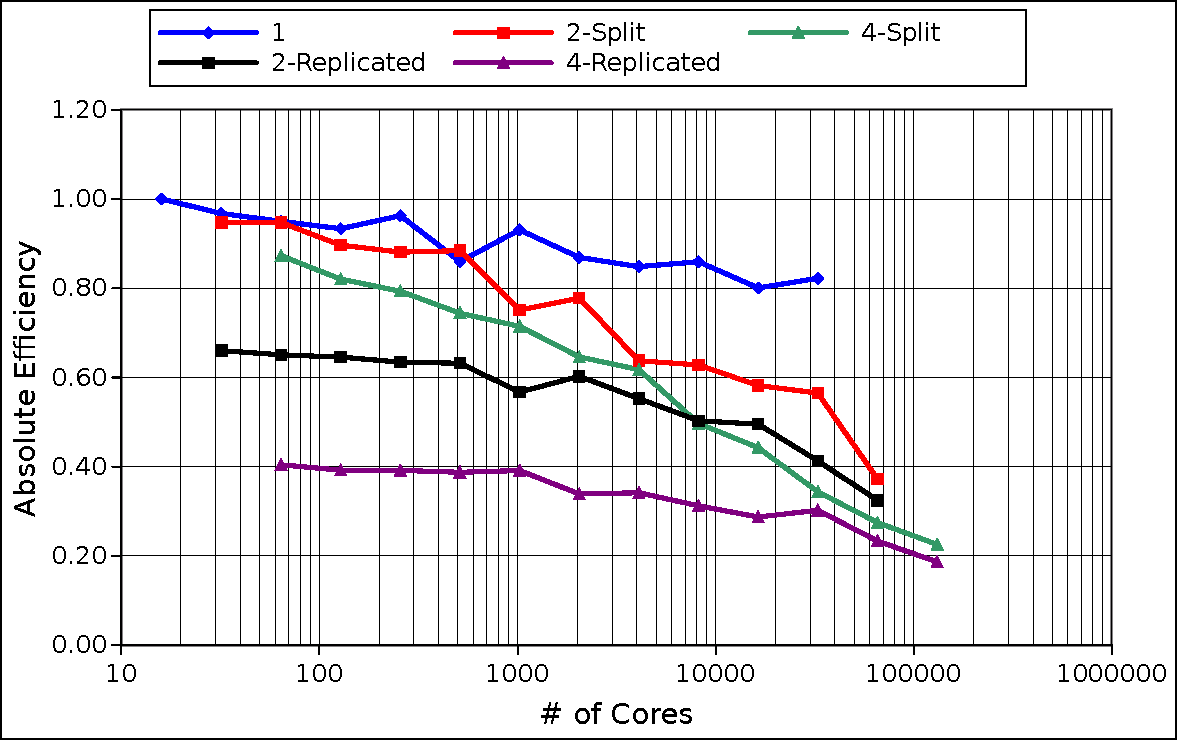
\includegraphics[width=6in]{chapters/parallel_mc/titan_weak_ms_eff.pdf}
  \end{center}
  \caption{\textbf{Weak scaling absolute efficiency relative to
      16-core 1-set base case.}}
  \label{fig:titan_weak_ms_eff}
\end{figure}

As in the strong scaling case, splitting and replicating histories
across sets had effectively the same results for the weak scaling
study with the iterations to converge and computed algorithmic
efficiencies given by Table~\ref{tab:ms_weak_alg_eff}. Again, when the
implementation efficiencies are computed, we see in
Figure~\ref{fig:titan_weak_ms_impeff} that splitting histories among
sets is still a more efficient manner of introducing multiple sets
rather than replicating histories in an attempt to reduce the number
of iterations required to converge.  Here we also note that this is
not a true weak scaling study as indicated by
Eq~(\ref{eq:ms_weak_efficiency}) but rather an odd combination of both
weak and strong scaling. Regardless of this, although multiple sets
are not the most efficient use of resources in this analysis, they do
enhance the time to solution through replication and do so
significantly at core counts of O(1,000) and lower. In both the weak
and strong scaling cases, due to the additional computational and
communication overhead of adding sets to the system, one should never
expect to seriously boost parallel efficiencies for MCSA using this
technique except for certain instances past the strong scaling wall in
a purely strong scaling environment. In a weak scaling environment,
although no efficiency increase will be noted, one can expect an
enhancement of time to convergence by replicating.

\begin{table}[h!]
  \begin{center}
    \begin{tabular}{lcc}\hline\hline
      \multicolumn{1}{l}{Case}& 
      \multicolumn{1}{c}{Iterations}&
      \multicolumn{1}{c}{$\eta_{alg}$} \\\hline
      1 & 22 & 1.0 \\
      2-split & 22 & 1.0 \\
      2-replicated & 16 & 1.375 \\
      4-split & 22 & 1.0 \\
      4-replicated & 13 & 1.692 \\
      %%
      \hline\hline
    \end{tabular}
  \end{center}
  \caption{\textbf{Weak scaling algorithmic efficiency using multiple
      sets.} \textit{Replicating histories improves algorithmic
      efficiency by converging in fewer iterations.}}
  \label{tab:ms_weak_alg_eff}
\end{table}

\begin{figure}[t!]
  \begin{center}
    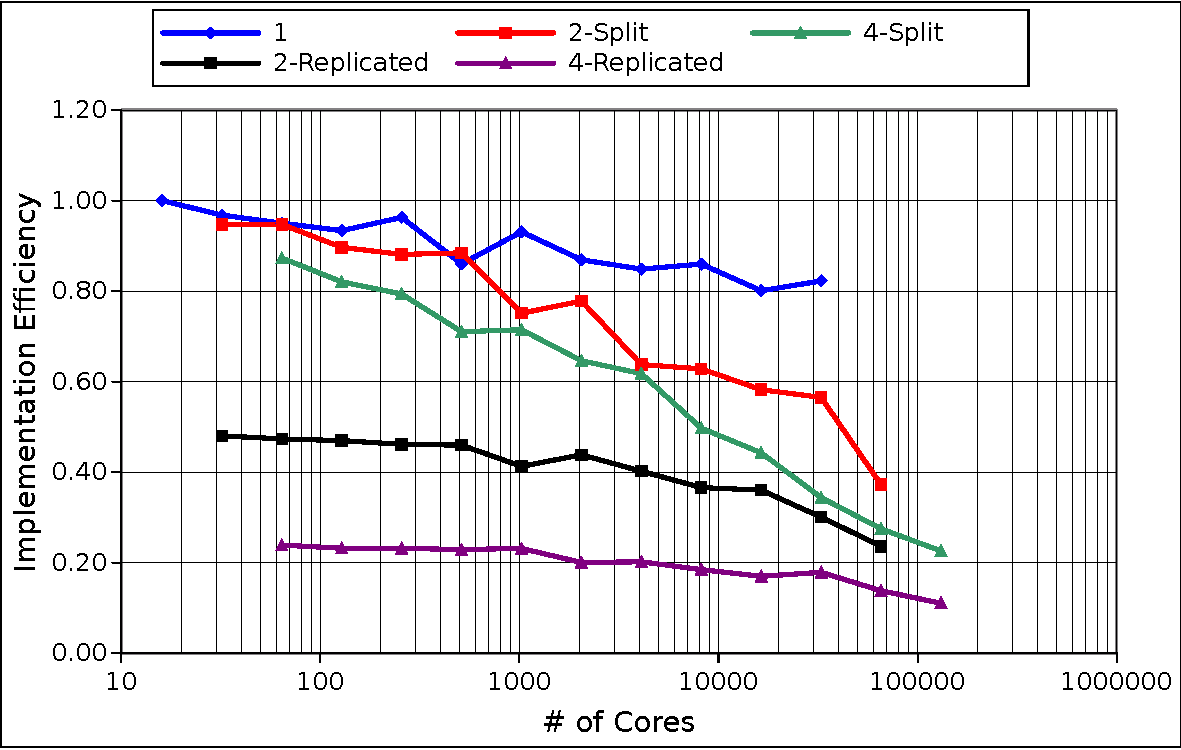
\includegraphics[width=6in]{chapters/parallel_mc/titan_weak_ms_impeff.pdf}
  \end{center}
  \caption{\textbf{Implementation parallel efficiency relative to 16-core
      1-set base case.}}
  \label{fig:titan_weak_ms_impeff}
\end{figure}

\clearpage

\subsection{Subdomain Neumann-Ulam}
\label{subsec:full_clip}

Based on the analysis of the pure domain decomposed MCSA algorithm and
subsequently the multiple sets and overlapping domain implementation,
one may ask then ask if there is any need to communicate histories
from domain-to-domain at all. Overlap was not as successful because
because the additional communication required to reduce the
overlapping tally vector eventually becomes larger than the
communication savings during Monte Carlo transport. In addition, for
local domains that are large enough to get good performance
(e.g. those used in the weak scaling studies), then our analytic
relationships for domain leakage, and in particular
Eq~(\ref{eq:mean_chord_domain_leakage}), tell us that only about 5\%
of the histories in this diffusion problem will leave the domain in
the first place.  If that is true, then perhaps without any overlap or
communication, just doing local Monte Carlo transport such that
histories are terminated upon reaching the domain boundary may be
satisfactory for accelerating the MCSA iteration. In this case,
histories near the boundaries of the domain may be truncated before
reaching the weight cutoff if they reach the domain boundary
first. This truncation has the potential to increase the stochastic
uncertainty of the Neumann-Ulam result and therefore increase the
number of MCSA iterations required to converge. In addition, the
scalability of the method will then be purely limited by the parallel
matrix and vector operations required to implement the remainder of
the algorithm on the subset of processors containing the linear
problem.

Considering using MCSA in this way such that the Monte Carlo solve
occurs only in the subdomains casts the method as more of a true
domain decomposition as outlined by Chapter 14 of Saad's text on
iterative methods \cite{saad_iterative_2003}. Compared to traditional
domain decomposition methods we see many similarities including the
potential to overlap the subdomains to improve the results. By
building the boundary data as outlined in
\S~\ref{subsec:domain_generation}, we are effectively gathering one
level of the adjacent domains, albeit in this case to satisfy the data
requirements of the Monte Carlo estimators. Furthermore, the fact that
we are using residual Monte Carlo to compute the correction vector
casts MCSA as a stochastic realization of an additive Schwarz method
with a fixed point iteration used as a relaxation step\footnote{See
  section 14.3.3 in \cite{saad_iterative_2003} for a full definition
  of the additive Schwarz method.}. Both the fixed point iteration and
the computation of the residual propagate the solution from individual
subdomains to the others through the matrix-vector multiply operation
after all subdomain Monte Carlo solves have been completed. Perhaps an
even more important consequence of viewing MCSA as a stochastic
additive Schwarz procedure is that it has the potential to more
readily fit as an accelerator into other linear solver techniques
including GMRES or potentially as a preconditioner.

Using the Neumann-Ulam solver to compute the MCSA correction only in
the subdomains, the strong and weak scaling studies were repeated to
assess the performance gains made by eliminating communication in the
Monte Carlo solver. For each scaling study, the 16-core base case with
Monte Carlo communication was used as the reference point for
efficiency computations in order to measure how eliminating
communication boosts
efficiencies. Figure~\ref{fig:titan_strong_subdomain} gives the
results of the strong scaling study and
Figure~\ref{fig:titan_weak_subdomain} gives the results of the the
weak scaling study in terms of absolute efficiencies. In both cases,
the benefits to parallel performance of using MCSA as a subdomain
solver are obvious. In the strong scaling case we make the important
observation that we hit the strong scaling wall at the same time with
and without the additional Monte Carlo communication. Although the
Monte Carlo communication did contribute to the efficiency decrease,
it is clear that the remaining matrix and vector operations are the
primary impediment to scalability. Furthermore, we see an even greater
rise above unity in efficiencies because there is less communication
overhead hiding the better cache utilization as the local problem size
shrinks. At 16,384 cores, performing the subdomain solves boost the
absolute efficiency from 38\% to 67\% relative to the reference case.

In the weak scaling study, we do not have the scaling wall to contend
with and eliminating Monte Carlo communication through subdomain
solves provides an effectively linear boost in the weak scaling
absolute efficiency. We still see a small reduction in weak scaling
efficiency as a function of core count due to the communication
overhead for the parallel matrix and vector operations. Here we
observe super unitary efficiencies for the subdomain case as there was
a substantial improvement in runtimes relative to the 16-core base
case with Monte Carlo communication.

\begin{figure}[t!]
  \begin{center}
    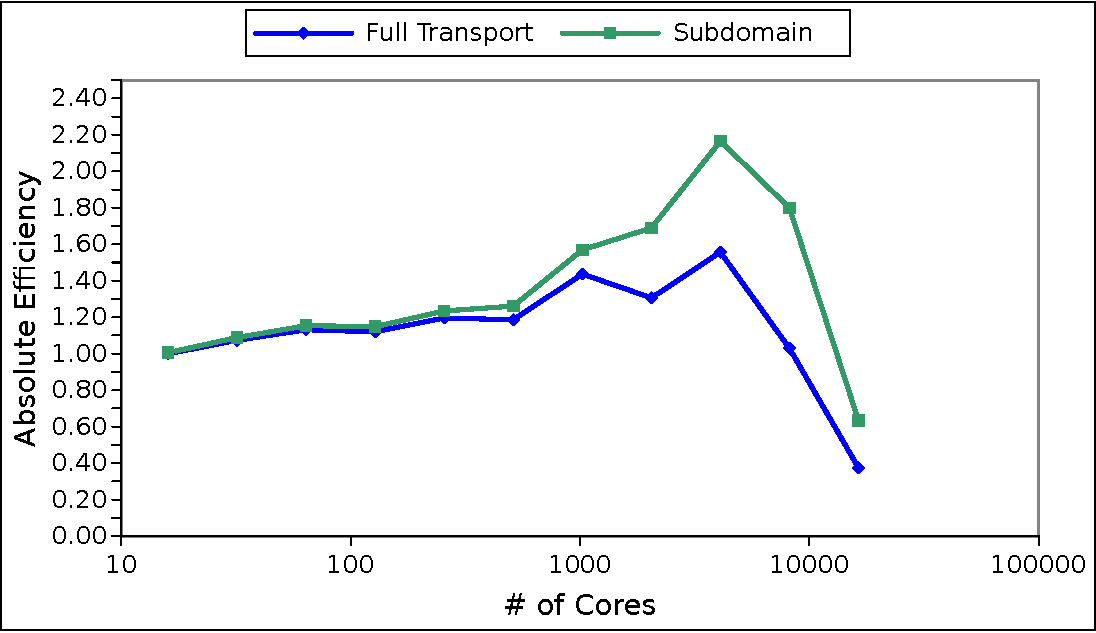
\includegraphics[width=6in]{chapters/parallel_mc/titan_strong_subdomain.pdf}
  \end{center}
  \caption{\textbf{Strong scaling absolute efficiency for pure domain
      decomposition.} \textit{The subdomain Monte Carlo solver
      improves the parallel efficiency and therefore time to solution
      by eliminating all parallel communication during the Monte Carlo
      solve.}}
  \label{fig:titan_strong_subdomain}
\end{figure}

\begin{figure}[t!]
  \begin{center}
    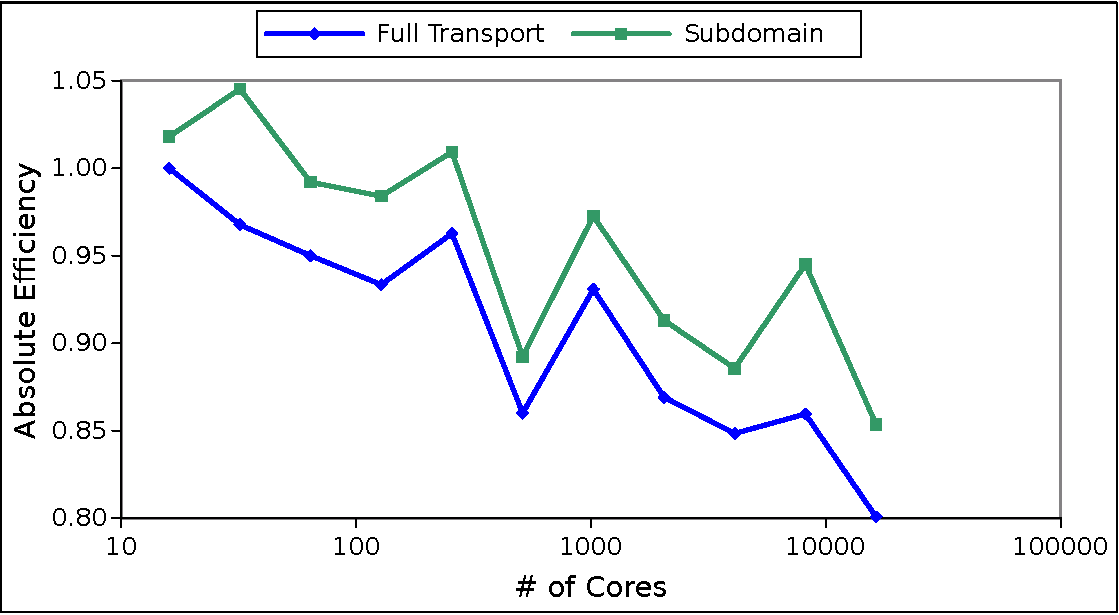
\includegraphics[width=6in]{chapters/parallel_mc/titan_weak_subdomain.pdf}
  \end{center}
  \caption{\textbf{Weak scaling absolute efficiency for pure domain
      decomposition.} \textit{The subdomain Monte Carlo solver
      improves the parallel efficiency and therefore time to solution
      by eliminating all parallel communication during the Monte Carlo
      solve.}}
  \label{fig:titan_weak_subdomain}
\end{figure}

Of additional concern for the subdomain method is the potential
decrease in iterative performance due to the fact that histories near
the boundary will potentially have their random walk truncated, thus
decreasing the information available to compute the correction
vector. For both the weak and strong scaling study, all calculations
with split histories converged in 22 or in only a few cases 21
iterations for both the subdomain solve and the solve with
communication giving an algorithmic efficiency of 1.048 for all
cases. This small improvement in iteration count was not observed to
be a function of problem size, number of processors, or whether the
subdomain method was used. For the replicated history cases, the
algorithmic efficiency improvement was not as good as when
communication was allowed for the Monte Carlo algorithm. For these
calculations, the number of iterations to converge was reduced to 18
or 19 in both the strong and weak scaling studies with lower core
counts converging in fewer iterations.

Therefore, there is no reason to expect overlap to improve the
iterative or scaling performance of the method as iterative
performance is maintained without it for this particular
problem. Overlap is not as effective because histories relinquish most
of their useful information within the first few steps (which is why
we can use such a large weight cutoff and there is an insensitivity to
weight cutoff as shown in
Figure~\ref{fig:estimator_wc_iters}). Keeping them around longer with
overlap to do extra work in the local domain will not improve
iterative performance and thus increase compute times.

As a final analysis of MCSA using subdomain Monte Carlo, the multiple
sets scaling studies are repeated to determine if any performance
benefits are made from replication by eliminating Monte Carlo
communication. Figure~\ref{fig:titan_strong_subdomain_ms_time} gives
the runtimes for the strong scaling calculation and
Figure~\ref{fig:titan_strong_subdomain_ms} the computed absolute
efficiencies. For the weak scaling studies,
Figure~\ref{fig:titan_weak_subdomain_ms_time} gives the wall times and
Figure~\ref{fig:titan_weak_subdomain_ms} the efficiencies. For both
scaling studies, the results are effectively the same as for the case
with Monte Carlo communication. This is again due to the fact that
adding sets to the problem is not only an exercise in strong scaling
but it also adds additional parallel overhead in the form of the tally
vector reduction across blocks.

From a parallel performance perspective, MCSA may then be best used in
a mode where the Monte Carlo is performed over only the subdomains
with no replication or overlap added to the system. In this mode,
iterative performance is maintained relative to the solutions with
communication even for more ill-conditioned problems with larger
spectral radii. Furthermore, no overlap was required to maintain
iterative performance be letting histories near the boundary take a
few more steps in their random walks. If in the future there are
ill-conditioned problems where using subdomain Monte Carlo reduces the
algorithmic efficiency of MCSA due to the information lost in the
correction vector, overlap would be a viable mechanism to potentially
maintain that iterative performance, keeping in mind the potential
impacts on scalability that were observed in this work. However,
although eliminating all Monte Carlo communication was observed to be
the best mode of use for MCSA, the parallel Monte Carlo methods
developed for this work still provide value for cases where only a
Monte Carlo solution is desired. In those cases, full transport of the
Monte Carlo histories are required in order to generate the correct
solution.

\begin{figure}[t!]
  \begin{center}
    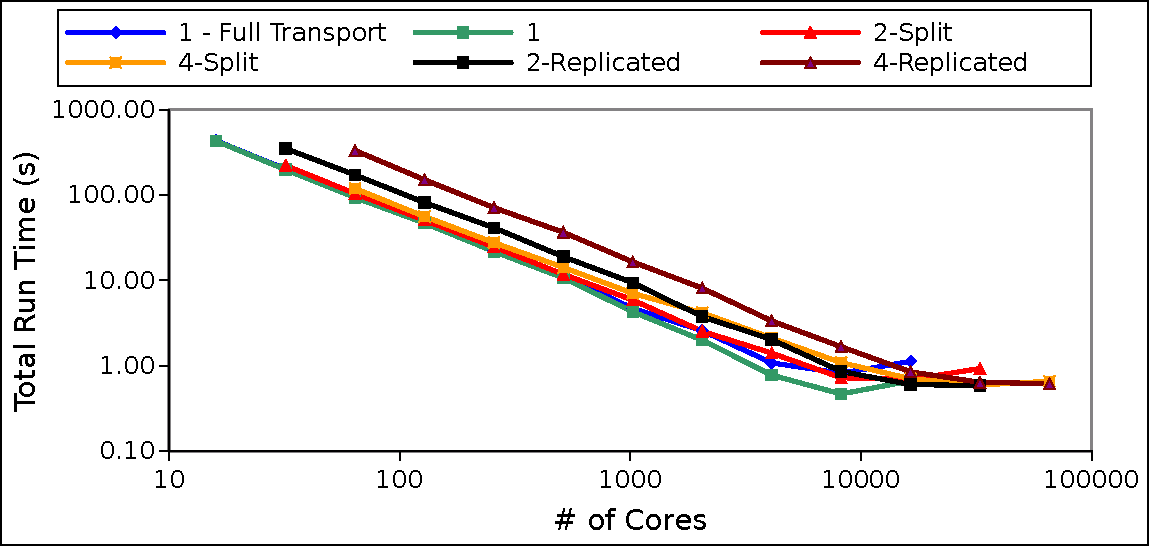
\includegraphics[width=6in]{chapters/parallel_mc/titan_strong_subdomain_ms_time.pdf}
  \end{center}
  \caption{\textbf{Strong scaling total wall time with multiple sets
      and subdomain Monte Carlo.} \textit{Adding multiple sets has in
      general a negative effect on the wall time as was observed for
      the case with full Monte Carlo transport.}}
  \label{fig:titan_strong_subdomain_ms_time}
\end{figure}

\begin{figure}[t!]
  \begin{center}
    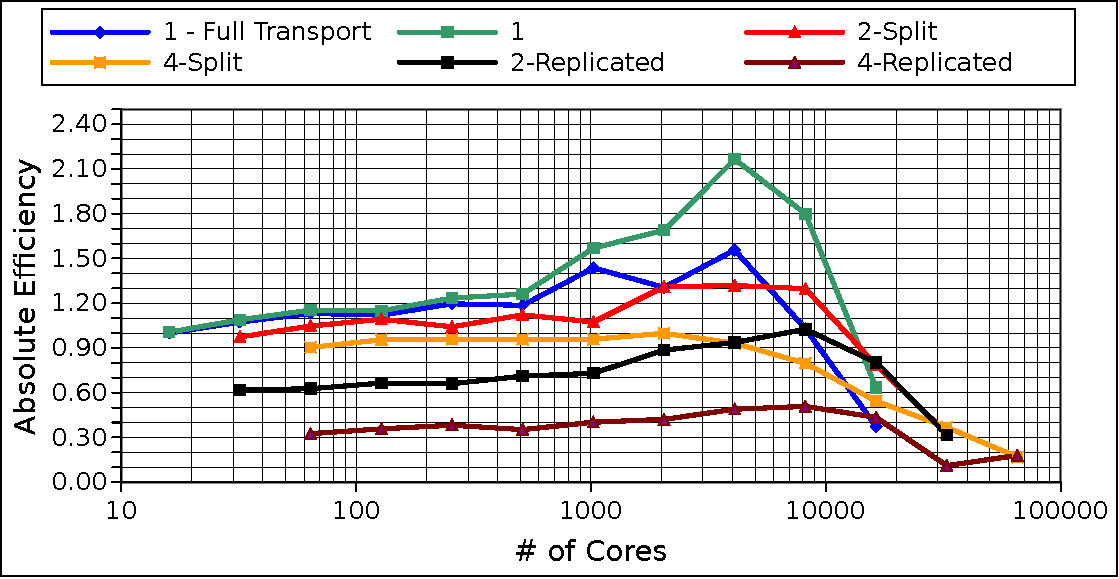
\includegraphics[width=6in]{chapters/parallel_mc/titan_strong_subdomain_ms.pdf}
  \end{center}
  \caption{\textbf{Strong scaling absolute efficiency for with
      multiple sets and subdomain Monte Carlo.} \textit{Increased wall
      times from adding parallel reduction operations for multiple
      sets reduces parallel scalability at lower core counts but gives
      a higher efficiency at the strong scaling wall.}}
  \label{fig:titan_strong_subdomain_ms}
\end{figure}

\begin{figure}[t!]
  \begin{center}
    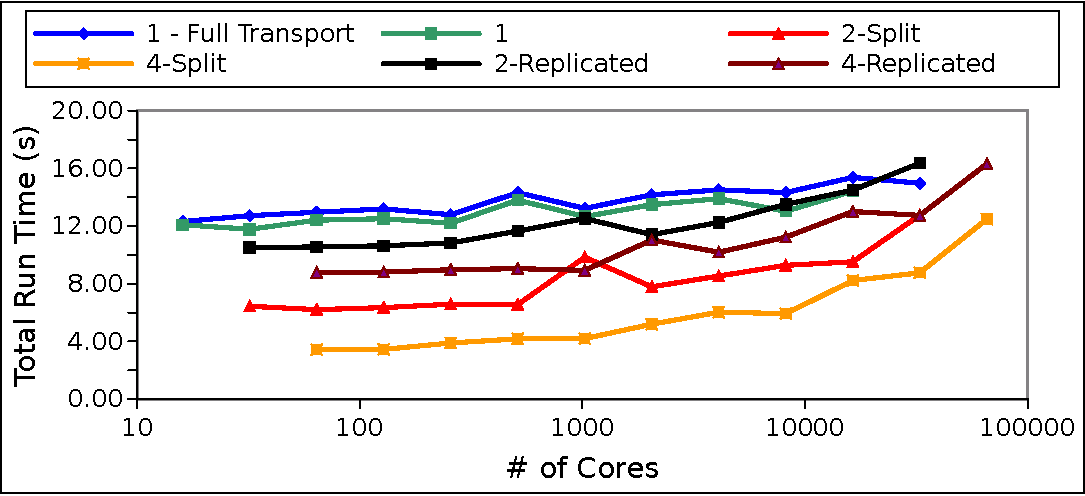
\includegraphics[width=6in]{chapters/parallel_mc/titan_weak_subdomain_ms_time.pdf}
  \end{center}
  \caption{\textbf{Weak scaling total wall time with multiple sets and
      subdomain Monte Carlo.} \textit{The addition of the set tally
      reduction is significant with cost of the reduction observed as
      core count grows.}}
  \label{fig:titan_weak_subdomain_ms_time}
\end{figure}

\begin{figure}[t!]
  \begin{center}
    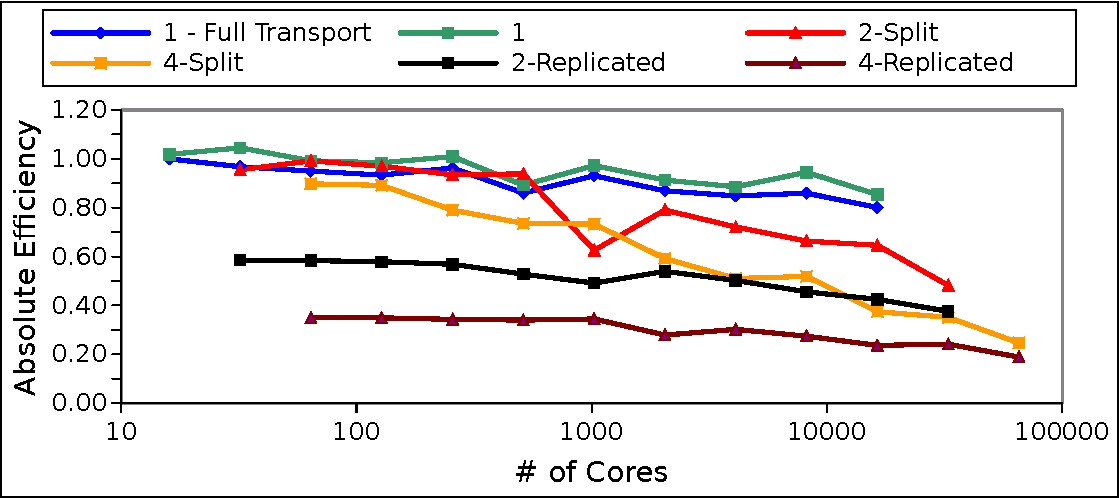
\includegraphics[width=6in]{chapters/parallel_mc/titan_weak_subdomain_ms.pdf}
  \end{center}
  \caption{\textbf{Weak scaling absolute efficiency for with multiple
      sets and subdomain Monte Carlo.} \textit{Weak scaling
      efficiencies are not improved at large core counts when multiple
      sets are added.}}
  \label{fig:titan_weak_subdomain_ms}
\end{figure}

\clearpage

%%---------------------------------------------------------------------------%%
\section{Summary\ }
\label{sec:parallel_summary}

In this chapter we have developed a domain-decomposed parallel
algorithm for Monte Carlo Synthetic Acceleration and explored the
qualities of the algorithm through parallel scaling studies. The
following are the significant observations and findings.

\begin{itemize}
\item MCSA can be effectively parallelized using domain decomposition
\item The leakage fraction of stochastic histories from a parallel
  subdomain can be quantified analytically using algebraic quantities
\item The multiple-set overlapping-domain (MSOD) parallel algorithm
  for particle transport has been adapted to parallelize MCSA
\item MCSA parallelized with MSOD was verified to produce the same
  results for solutions to the neutron diffusion equation as
  production Krylov methods
\item Strong scaling studies were performed with up to 65,536 cores
  and weak scaling studies were performed with up to 131,072 cores on
  the Titan Cray XK7 leadership class machine at Oak Ridge National
  Laboratory
\item MCSA scales favorably compared to production Krylov methods for
  both strong and weak scaling cases
\item Overlap in small quantities determined analytically by random
  walk length can provide parallel efficiency boosts of a few percent
  in strong scaling cases but is ineffective in weak scaling cases
\item Multiple sets will never boost parallel efficiencies in the weak
  scaling case due to additional communication overhead from added
  reduction operations but will boost efficiencies beyond the strong
  scaling wall
\item Multiple sets offers a means to reduce time to solution by
  solving multiple copies of the original problem and combining the
  solutions using superposition
\item MCSA is most efficiently used in parallel as a stochastic
  realization of an additive Schwarz method
\item With future optimization, large scale reactor analyses in which
  the transport operator is fully formed (e.g. the $SP_N$ equations)
  could experience improved time to solution on leadership-class
  machines with MCSA given the improved scaling performance
\end{itemize}
